\documentclass{article}
\usepackage{graphicx} % Required for inserting images
\usepackage[left=3cm, right=3cm, top=3cm, bottom=3cm]{geometry}
\usepackage{hyperref}
\usepackage{url}
\usepackage[titles]{tocloft}
\usepackage{amsmath}

\usepackage{listings}
\usepackage[dvipsnames]{xcolor}
%\usepackage{amsmath}
\usepackage{mdframed}

\renewcommand{\lstlistlistingname}{Code Snippets}

\newcommand{\dd}{\ensuremath{\mathrm{d}}}
\newcommand{\diff}[2]{\ensuremath{\frac{\dd {#1}}{\dd {#2}}}}
\newcommand{\bv}[1]{\ensuremath{\mathbf{#1}}}
\newcommand{\ls}[1]{\lstinline{#1}}

\definecolor{codegreen}{rgb}{0,0.6,0}
\definecolor{codegray}{rgb}{0.5,0.5,0.5}
\definecolor{codepurple}{rgb}{0.58,0,0.82}
\definecolor{backcolour}{rgb}{0.95,0.95,0.92}
\definecolor{exercise}{gray}{0.9}
\definecolor{SIM}{cmyk}{0.1, 0, 0, 0}

\newcounter{exercise}
\newenvironment{exercise}[1][]%
    {\refstepcounter{exercise}%
    \begin{mdframed}[backgroundcolor=exercise,linecolor=white]%
    \textbf{Exercise~\theexercise.} #1 \rmfamily}%
    {\medskip\end{mdframed}}

\newcommand{\listsyntax}{Python Language Intermezzos}
\newlistof{intermezzos}{synt}{\listsyntax}
\newcounter{syntax}
\newenvironment{syntax}[1][Syntax]%
    {\refstepcounter{syntax}%
    \addcontentsline{synt}{intermezzos}{#1}
    \begin{mdframed}[backgroundcolor=SIM,linecolor=white]%
    \textbf{Intermezzo~\thesyntax:} \textit{#1}}%
    {\medskip\end{mdframed}}

\lstdefinestyle{py}{
    backgroundcolor=\color{backcolour},
    commentstyle=\color{codegreen},
    keywordstyle=\color{magenta},
    numberstyle=\tiny\color{codegray},
    stringstyle=\color{codepurple},
    basicstyle=\ttfamily\footnotesize,
    breakatwhitespace=false,
    breaklines=true,
    captionpos=b,
    keepspaces=true,
    numbers=left,
    numbersep=5pt,
    showspaces=false,
    showstringspaces=false,
    showtabs=false,
    tabsize=2,
    language=Python
}
\lstset{style=py}

\title{NOFY080 lecture notes}
\author{Emil Varga}
\date{\today}

\begin{document}

\maketitle

\tableofcontents
\listofintermezzos
\lstlistoflistings

\newpage
\section{A quick introduction to basic Python}

\subsection{Running Python code}
Python is an interpreted language that does not need to be compiled before it is run. We save Python code in text files with \verb|.py| file extension or in so-called Jupyter notebooks (file extension \verb|.ipynb|).

To run a Python code, open a suitable terminal (on Windows with Anaconda distribution of Python this will be \verb|Anaconda prompt|) and type in \verb|python| a prompt like
\begin{lstlisting}
    >>>
\end{lstlisting}
will appear. This is the Read-Evaluate-Print-Loop (REPL), any code entered will be run and the result printed on the screen. To exit enter \verb|quit()|. To execute a file \verb|myfile.py|, first navigate to its directory and then run it simply with \verb|python myfile.py|.

\begin{exercise}
    Create a textfile \verb|hello.py| which contains a single line
    \begin{lstlisting}
        print("Hello world!")
    \end{lstlisting}
    and then run this file.
\end{exercise}

Sometimes we do not want the Python interpreter to quit immediately after finishing running our program (e.g., we want to inspect variables created during the program run), this can be done using \verb|python -i file.py|, \verb|-i| stands for \emph{interactive}. Alternatively, a more user-friendly (color-coded syntax, auto-completion, etc.) version of the interactive python REPL can be invoked using \verb|ipython| (or \verb|ipython3|, depending on your installation), which can also be used to interactively run files using \verb|ipython3 -i myfile.py|

\subsubsection{A quick note on text editors}
Any text editor can be used to write Python code, including the default Windows Notepad. However, it is beneficial to your mental health to use at least something with syntax highlighting, such as Notepad++, or a more feature-rich editor such as VS Code or Spyder where you can run your file without switching to a terminal. In this course, I will be using Spyder, but almost nothing in the course will be exclusive to it.

\subsubsection{Jupyter Notebooks}
Jupyter notebooks (run using \verb|jupyter-notebook| in the command line) provide an easy-to-use interactive environment with an interface running in a web browser. Good for trying things out. \footnote{In this course we will be (mostly) using scripts due to easier splitting to modules and fewer issues with parallel programming, which we will encounter later on.}

\subsection{Variables and types}

Variables are created by assigning a value to an unused variable name, declarations, such as in C/C++ or Pascal are not necessary
\begin{lstlisting}[caption=Defining variables]
    my_integer = 5
    my_float = 3.14
    my_string = "double quote string"
    my_string2 = 'single quote string'
    my_string3 = "you can use 'single' quote in double quote string"
    my_bool = False
\end{lstlisting}

Note that variables generally do not have a fixed type (i.e., an integer or a string), and doing something like \lstinline{my_integer = "a string"} will not result in type error. Python itself does not care about what type the variable is as long as the operations we do with it are supported. However, if we need to know the type of a variable \lstinline{v} we can find it using \lstinline{type(v)}.

Basic arithmetic operations \verb|+,-,*,/| work as expected on numbers. Exponentiation is \verb|**|. Note, however, that \verb|/| automatically \emph{promotes} integers to float. For integer division, we can use \verb|//| and for the remainder \verb|%|. Arithmetic operations are also defined for some non-number types where they "make sense", i.e., strings can be concatenated using \verb|+|. Comparison operators are \verb|==| for equality (\textbf{not to be confused with =, which is the assignment of a value to a variable}), \verb|!=| for inequality and \verb|<,<=,>,>=| for ordering. Boolean operators are \verb|and, or, not|. 

There are also \textbf{bitwise} operators \lstinline{&,|,~,^} (bitwise AND, OR, NOT and XOR, respectively). These operate on individual bits of a number. Careful about the confusion between exponentiation \ls{**} and bitwise exclusive or \ls{^}.

Complex numbers are supported in Python. The syntax to specify a complex number is, e.g., \ls{3 + 5j}, which translates to mathematical $3 + 5i$. Specifically, the imaginary unit is \ls{1j}. Notice that the letter \ls{j} follows the number immediately.

\begin{exercise}
    Try out the basic arithmetic in REPL. Try multiplying a string by an integer. What happens when you try dividing?
\end{exercise}

A summary of basic built-in operators

\begin{tabular}{ll}
     \ls{+,-,*,/, **} & basic arithmetic, exponentiation \\ 
     \ls{and, or, not} & boolean operations \\
     \ls{<, <=, ==, >, >=} & comparison\\
     \ls{&,|, ~, ^} & bitwise operations, bitwise AND, OR, NOT and XOR (exclusive or)
\end{tabular}

\subsection{User input}
We will be mostly writing non-interactive scripts, however, to get basic text-based input from the user we can the \verb|input()| function, \textbf{which always returns a string}. We have to convert it to a number (using \verb|int()| or \verb|float()|) ourself if that is what we expect the user to enter, e.g.,
\begin{lstlisting}
    age = int(input("How old are you? "))
    print("You will be 100 in", 100-age, "years.")
\end{lstlisting}

\subsection{Printing and strings}
We have already met function \verb|print()|, which prints a text representation of whatever objects pasted to it to standard output. It accepts one or more arguments.

To turn any value to a string we can use the function \verb|str()|. Special characters, such as new line or tab, need to be \emph{escaped}, e.g., \verb|\n| and \verb|\t|, respectively. Backslashes also need to be escaped \verb|\\|. To stop python from trying to interpret backslashes as special characters (useful, e.g., for specifying file paths on Windows) we can use raw strings, e.g.,
\begin{lstlisting}
    print("s\tri\ng") #\t and \n are interpreted as tab and new line
    print(r"s\tri\ng") # raw string, note the r immediately before "
\end{lstlisting}

For crafting more complicated way of printing our variables we can use \emph{format} strings (or f-strings) by enclosing the variable we wanted inserted into the string in \verb|{}|, e.g.,
\begin{lstlisting}
    vari = 5
    varf = 3.14
    fstr = f"An interger value {vari:05d}, a float value {varf:010.6f}, exponential form {varf:g}"
\end{lstlisting}
The variable substitution is specified as \verb|{expression:format_specifier}|, the format specifiers are optional. Here the format specifier 05d means a decimal integer with total width of at least 5 characters and 010.6f means floating point number with 6 digits after the decimal period and total width of at least 10 characters.

For a full specification of possible format specifiers see \url{https://docs.python.org/3/library/string.html#formatspec}

\subsection{Functions}
Functions are defined using the \verb|def| keyword. Functions may take argument and return a value.
\begin{lstlisting}
    def my_function(my_string):
        print("Someone wants to know how long \"" + my_string + "\" is!")
        return len(my_string) #returns the length of a my_string
\end{lstlisting}
Note the indentation, which is how blocks of code are identified in Python, i.e. there is no \verb|begin,end| as in Pascal or \verb|{}| as in C/C++.

Multiple arguments are separated with a comma and arguments can have a default value, e.g. the argument $c$ will be 1 unless specified
\begin{lstlisting}[caption=Function definition]
    def calculate(a, b, c=1):
        """
        A function that calculates c*(a + b)

        Parameters:
        -----------
        a, b, c: numbers
            arguments of the calculation

        Returns:
        --------
        result: number
            The result of calculating c*(a + b)
        """
        return c*(a + b)

    >>> calculate(2, 3)
    5
    >>> calculate(2, 3, 4)
    20
\end{lstlisting}
Here the long string delimited by triple quotes \lstinline{"""} is the so-called documentation string of the function (or \textbf{docstring} for short). Triple quotes can be used anywhere and indicate only that the string span multiple lines. The docstring then can be accessed using the \lstinline{help()} function or by text editors. The formatting used in the above example is commonly understood by IDEs, e.g., Spyder will display it nicely formatted in the Help pane (upper right corner of the window by default).

Arguments with default values must come after the required arguments. With multiple optional arguments we can call the function using \emph{keyword arguments}:
\begin{lstlisting}[caption=Optional and keyword arguments.]
    def calculate2(a, b, c=1, d=1):
        return c*(a + b)**d

    >>> calculate(2, 3, d=2) # leaves c default, but specifies d
    25
\end{lstlisting}

Functions can be passed around in variables and arguments, specifically, functions can accept other functions as arguments, e.g.,
\begin{lstlisting}[caption=Higher order functions.]
    def add1(x):
        return x + 1

    def change_number(x, func):
        return func(x)

    >>> change_number(1, add1)
    2
\end{lstlisting}

Short, simple functions (that fit on one line) can be defined in-line as so-called anonymous, or \emph{lambda}, functions, e.g.
\begin{lstlisting}[caption=Lambda functions.]
    >>> changer_number(1, lambda x: 2 + x)
    3
\end{lstlisting}
Lambdas are especially useful for partially filling out argument lists of existing functions, e.g.
\begin{lstlisting}
    >>> change_number(1, lambda x: calculate2(x, 4, c=4, d=0.5))
    8.94427190999916
\end{lstlisting}

\subsection{Compound types}

\subsubsection{Lists and tuples}
A \textbf{list} is a collection of any python objects defined using square brackets \verb|[]|,
\begin{lstlisting}
    my_list = [1, 2.17, "a string", ['another', 'list']]
\end{lstlisting}
The values in the list can be accessed by indexing the list \textbf{starting from 0}, e.g., \verb|my_list[1] == 2.17|. Negative indices count from the back, i.e., \verb|my_list[-1]| is the last element, \verb|my_list[-2]| second-to-last etc.

Lists are an example of an \emph{object}, objects have associated functions called methods, which are called with a dot syntax. Useful methods for lists are
\begin{itemize}
    \item \verb|append| and \verb|pop|
\begin{lstlisting}
>>> my_list = [1, 2.0, 'three']
>>> my_list.append('one more')
>>> my_list.pop() # removes the last element and returns it
"one more"
\end{lstlisting}
    \item \verb|my_list.sort()|, sorts the list in-place if all elements of the list can be compared; to create a new list with sorted elements we can use \verb|sorted(my_list)|
    \item \verb|my_list.index('a')| finds the index of first occurence of 'a' or returns an error
\end{itemize}

Apart from simple indexing, subsets of lists can be accessed using \emph{slicing}, e.g.,
\begin{lstlisting}
    l = [1,2,3,4,5,6,7,8,9]
    l[2:5] # [3,4,5]
    l[-5::2] # [5,7,9]
\end{lstlisting}
Generally the syntax is \verb|my_list[start_idx:stop_idx:step]|, \verb|start_idx| is inclusive, \verb|stop_idx| is exclusive. All three are optional, start defaults to 0, stop defaults to -1 and step defaults to 1.

\textbf{Tuples} behave in many ways similarly to lists, with the exception that they are \textbf{immutable}, i.e., the tuple itself or the values in it cannot be changed. Indexing and slicing, however, work the same. Tuples are defined using ordinary brackets \ls{()}. If the tuple contains only one value a comma needs to be included to distinguish it from a bracketed expression, i.e., \ls{single_tuple = (1,)}.

A common use for tuples is to return multiple values from a function, i.e.,
\begin{lstlisting}
    def add_and_subtract(x, y):
        return x+y, x-y #note that the parentheses () are not required in return

    #here we unpack the return value into two variables
    a, s = add_and_subtract(3, 2) # a==5, s==1
\end{lstlisting}
Note that we did not store the return value as a tuple but immediately split it into two separate variables. This is called \textbf{unpacking} and can be used for any compound type.

\subsubsection{Dictionaries}
Dictionaries are a collection of assignments from a key to a value of any type, often the keys are strings e.g.,
\begin{lstlisting}
    my_dict = {
        'key1': value1
        'key2': value2
    }
\end{lstlisting}
which can then be accessed as \ls{my_dict['key2']} etc.


\subsection{Control flow}

\subsubsection{if-elif-else}
The \verb|if| statement takes a boolean expression and runs the code in its code block if the condition evaluates to \verb|True|.
\begin{lstlisting}[language=Python]
    if condition:
        do_if_true()
    elif condition2: #optional
        do_if_2true() #runs only if condition is False and condition2 is True
    else: #optional
        do_if_false() #runs only if both condition and condition2 are False
        
\end{lstlisting}

\subsubsection{match}
Available since Python 3.10
TODO
\begin{lstlisting}
    command = 'yell'
    match command:
        case 'talk':
            print("hello")
        case 'yell':
            print("HELLO!!")
        case _: #default behavior
            print("unknown command")
\end{lstlisting}

\subsection{Loops}
To loop for a given number of iteration we can use the \verb|for| loops with a \verb|range()| function. We can also loop over anything iterative, e.g., a list or dict.
\begin{lstlisting}
    for k in range(10):
        print(k)

    for value in my_list:
        print(value) 
\end{lstlisting}
The general form of \ls{range()} is \ls{range(start, stop, step)}, start is inclusive, stop is exclusive and step is by default 1. \ls{range()} does not return a list but something called an \emph{iterator}. We can turn it into a list using \ls{list(range(start, stop, step))}.

If we want to iterate over a list and we need to work with both the index and the value we can use \lstinline{enumerate}
\begin{lstlisting}
    for index, value in enumerate(my_list):
        print(f"my_list[{index}] = {value}")
\end{lstlisting}

To loop while a condition is true we can use the \verb|while| loop,
\begin{lstlisting}
    while condition:
        do_stuff()
\end{lstlisting}

Execution of loops can be modified using \ls{continue}, which skips the rest of the code in the iteration and goes to the next one or \ls{break} which immediately ends the loop. A common usage is with infinite loops, e.g.,
\begin{lstlisting}
    while True: # this will never end
        do_stuff()
        if should_we_stop: # unless we kill it
            break
\end{lstlisting}

Loops are often used to construct lists, which can be simplified using \textbf{list comprehension} such as
\begin{lstlisting}
    [expression(k) for k in iterable if condition(k)] # if condition is optional
\end{lstlisting}
For example,
\begin{lstlisting}[caption=List comprehension.]
    [k**2 for k in range(5)] # list of squares for k < 5
    [k**2 for k in range(5) if k % 2 == 0] # list of squares of even numbers
\end{lstlisting}

\begin{exercise}
    Write a program, which asks a user their name and replies \verb|"Hello <name>!"|.
    \begin{enumerate}
        \item Change the program such that if the user's name is "Andrej", the greeting changes to "Ciao Andrej!".
        \item Separate the logic of constructing the greeting to a separate function.
    \end{enumerate}
\end{exercise}
\begin{exercise}
    Write a program, which will accept arbitrary number of names from the command line and at the end prints them back in alphabetical order.
    \begin{enumerate}
        \item The user will enter beforehand the number of names they want to enter. \emph{Hint}: \verb|range()| and a \verb|for| loop
        \item The program will stop asking for new names once the user enters an empty string. \emph{Hint:} \verb|break|
        \item If the user entered the name "Emil", it will be skipped in the final output. \emph{Hint:} \verb|continue|.
    \end{enumerate}
\end{exercise}

\subsection{Using external modules}
Python is famous for having a large number of available libraries to do pretty much everything under the sun.\footnote{And we will learn how to create our own shortly.} To use these, we first need to import the \emph{module} we need, e.g. to use functions that deal with time we can do
\begin{lstlisting}
    import time as t #import the time module and gives it a shorthand name t
    print(t.time()) #we prepend the module name to the function to call it
\end{lstlisting}
If there is only a small number of functions we want to use from a given module we can import them specifically and don't have to use the module name to call them, e.g.
\begin{lstlisting}
    from module import func1, func2
    func1()
    func2()
\end{lstlisting}

\begin{exercise}
    Write a program to caluclate the Fibonacci number $F_n$ using both loops and recursion. Measure the time to calculate the first 20 $F_n$ using both methods using \verb|time.time()|.
    \emph{Hint:} $F_k = F_{k-1} + F_{k-2},\;F_1 = F_2 = 1$
\end{exercise}

\newpage
\section{NumPy, SciPy, and matplotlib}
\subsection{numpy}
These three libraries form the basis of many (probably most) of scientific Python scripts. NumPy provides a numpy array, a fast way of storing numerical data in memory, and functions to work with them. SciPy provides a large number of algorithms including least squares fitting, signal processing, or spatial clustering and matplotlib allows for the creation of high-quality and customizable plots. Both are designed to work with numpy arrays.

\begin{syntax}[Package installation -- pip]
    Packages that are not installed by default can be installed using a command line utility \ls{pip} which downloads packages registered in the Python Package Index (PyPI, \url{https://pypi.org/}). For example, the install the package \ls{lmfit} run the following command in the command line (also works in the ipython REPL, e.g., in Spyder)
    \begin{lstlisting}
        pip install lmfit
    \end{lstlisting}
    To remove the package use \ls{uninstall}, and to upgrade \ls{install -U}. Run \ls{pip help} for a complete list of available commands.
\end{syntax}

To use numpy we do
\begin{lstlisting}
    import numpy as np
\end{lstlisting}
there are several ways to create an array, e.g.
\begin{lstlisting}[caption=Array creation.]
    #directly from lists
    arr = np.array([1,2,3,4])
    #2D array
    arr_2D = np.array([[1,2,3],
                       [4,5,6],
                       [7,8,9]])
    # similar to list(range()), but none of the start, stop, or step have to be integers
    arr = np.arange(start, stop, step)
    #linearly spaced values
    arr = np.linspace(start, stop, count)
    #filled with zeros
    np.zeros(length)
    #filled with ones
    np.ones(length)
\end{lstlisting}

By default np arrays store type float. For ones and zeros it is often useful to use boolean values (True and False) as \lstinline{np.ones(10, dtype=bool)} will create an array of length 10 filled with True values. Arithmetic works on an element by element basis, therefore when we add/multiply/divide/compare the arrays must be the same length, e.g.,
\begin{lstlisting}
    >>> np.array([1,2,3]) + np.array([4,5,6])
    array([5,6,7])
\end{lstlisting}
However, if one of the operands is a scalar number, the operation \emph{broadcasts}, e.g.,
\begin{lstlisting}
    >>> np.array([1, 2, 3]) + 10
    array([11, 12, 13])
\end{lstlisting}

Array slicing works similarly to list slicing, e.g., \lstinline{arr[start:stop:step]}. Additionally, we can also index into an array using a list of indices, e.g., \lstinline{arr[[0, 2, 4]]} will return an array containing 1st, 3rd and 5th element of array \lstinline{arr}. Finally, using boolean arrays we can create an array subset of elements where the indexing array is true, e.g.,
\begin{lstlisting}
    arr1 = np.linspace(0, 10, 50)
    b = np.sqrt(arr1) > 3 # array of bools True where np.sqrt(arr1) > 3
    arr1[b] # only the elements of arr1 whose square root is larger than 3
\end{lstlisting}

\begin{exercise}
    Write a program that will (in a loop) add numbers $1 + 2 + 3 + ... + n$ for any $n$ using \verb|numpy| arrays and compare it with the Gauss' expression $n(n+1)/2$ for user-supplied $n$. \emph{Hint:} \verb|np.arange|
\end{exercise}
\begin{exercise}
    Write a function, which will return all prime numbers smaller than $N$ using the Sieve of Eratosthenes method. \emph{Hint:} \verb|enumerate()|, \verb|np.ones(N, dtype=bool)|, boolean array masking.
\end{exercise}

\subsubsection{Basic measures and operations with the arrays}
Since numpy arrays are intended primarily for numerical data, there are several methods built into them that calculate some basic measures, e.g.,

\begin{tabular}{lll}
\ls{arr.mean()} & mean of the array\\
\ls{arr.std()} & standard deviation, biased estimate of the variance\\
\ls{arr.sum(), arr.cumsum()} & the sum and cumulative sum\\
\ls{arr.max(), arr.min()} & maximum and minimum, respectively\\
\ls{arr.argmax(), arr.argmin()} & the index of maximum and minimum, respectively\\
\end{tabular}

As for any container type \ls{len(arr)}, returns the length of the array. These also exist in their function forms (e.g., we can call \ls{np.mean(arr)}). Additionally, there are useful functions that deal with arrays in the module itself: \ls{np.diff(arr)} returns an array of differences between nearest neighbors one shorter than \ls{arr}; for more general weighted averaging one can use \ls{np.average(arr, weights)}. Most of these functions have their corresponding nan- versions, which ignore NaN values in the arrays (e.g., \ls{np.nansum, np.nanmax} etc.). \ls{np.isnan(arr)} returns an array of the same length as \ls{arr} with True everywhere where \ls{arr} was NaN. For boolean-valued arrays the extension of \ls{and} and \ls{or} are \ls{np.logical_and(arr1, arr2)} and \ls{np.logical_or(arr1, arr2)} and similarly \ls{np.logical_not(arr)}, which create a new array with the logical operation applied to every element of the input arrays. Logical operators by themselves do not work with arrays.

\begin{syntax}[NaNs and Infs.]
     Mathematical operations can result in either a Not-a-Number (NaN) or infinities, which are represented in numpy by \ls{np.nan} and \ls{np.inf}. These are special values indicating, for NaN, that an undefined operation was performed, e.g., \ls{np.log(-1)} (Python and Numpy support complex numbers, but operations with real numbers are assumed to result in reals as well -- if we wanted to use the complex logarithm we would have to give it a complex -1, i.e., \ls{np.log(-1 + 0j)}).

    Simple division by zero, e.g., 1/0, will result in a ZeroDivisionError error. However, when part of an \ls{np.array} it will result in an $\pm$np.inf and a Warning, e.g., try running \ls{np.array(1)/np.array(0)}.

    The idea of not crashing on undefined operations or division by zero is in the idea that often only part of the array is damaged (e.g., a -1 can be a placeholder for a value that's not available) and it might be easier and cleaner to proceed assuming that all operations are valid and then simply throw out the NaNs at the end.
\end{syntax}

An array can be sorted in-place using \ls{arr.sort()} or a new sorted array can be created using \ls{sorted_arr = np.sort(arr)}. To get an array of indices that would sort the array we can use \ls{np.argsort()}, which is useful when we want to sort one array according to another, e.g.,
\begin{lstlisting}
    import numpy as np
    items = np.array(["Eggs", "Bread", "Apples"])
    prices = np.array([50, 20, 40])

    sort_ix = np.argsort(prices)
    print("Items sorted according to prices:")
    print(items[sort_ix])
\end{lstlisting}

\subsubsection{File I/O}
We will be using numpy and matplotlib to analyze some experimental data. First, we need to get the data, typically from some file on the disk. Assuming that we have data stored as a text file in \verb|data.txt| as two columns of numbers separated by tabs we can load it into a 2D numpy array using
\begin{lstlisting}
    arr = np.loadtxt("data.txt", comments='%', skiplines=3)
\end{lstlisting}
which loads \verb|data.txt| into 2D array \verb|arr|, ignores all lines beginning with \% and skips first three datalines. If, rather than tabs our data is separated by commas (i.e., a \verb|.csv| file) we can add a keyword argument \verb|delimiter=','| or use \lstinline{np.loadcsv()}.

\begin{syntax}[Paths]
    Paths to files or directories can be absolute or relative. Absolute path specifies the absolute position of a file in the filesystem, on Windows it will typically begin with something like \verb|C:\| and on Linux or Mac with the root directory \verb|/|.

    A relative path is relative to the current working directory, which can be obtained using \ls{getcwd()} from the \ls{os} module.

    Different operating systems use different directory separators, i.e., Windows uses \verb|\|, Linux and Mac \verb|/| and Japanese Windows computers use \verb|¥|. To join directory names in a way that will work everywhere we can use \ls{os.path.join('dir1', 'dir2', 'dir3', ...)}.

    To find multiple files whose name fit a pattern we can use the function \ls{glob()} from the module \ls{glob()}. For example, \ls{glob(os.path.join("photos", "photo*.png"))} will return a list of all files that fit the pattern \ls{"photos/photo<any number of any characters>.png")}
\end{syntax}

Using the file I/O functions from Python standard library is also possible. The function \lstinline{file = open(filename, mode)} opens the file in a given mode, most common are \lstinline{'r'} for reading, \lstinline{'w'} for (over)writing, and \lstinline{'a'} for appending. All contents of the file can be read in one go using \lstinline{file.readlines()} or we can iterate over the lines of the file using a for loop (see example below). Inversely, there is \lstinline{file.write(some_string)} (if the file is opened with mode 'r' this will fail). Especially for writing, it is important to call \lstinline{file.close()} after we are done with the file otherwise the changes might not be written to the disk due to caching.

The \lstinline{np.loadtxt()} with default arguments is roughly equivalent to
\begin{lstlisting}
    import numpy as np
    def my_load(fn):
        with open(fn, 'r') as file:
            rows = []
            for line in file:
                row = [float(s) for s in line.strip().split()]
                rows.append(row)
        return np.array(rows)
\end{lstlisting}
\begin{syntax}[with statement (basic)]
\lstinline{with} is an example of so-called context management which ensures that resources (in this case a file) are properly cleaned up after we are done using them. We will learn how to create our own context managers later, for now, the code
\begin{lstlisting}
    with open(fn, 'r') as file:
        do_stuff()
\end{lstlisting}
    is roughly equivalent to
\begin{lstlisting}
    file = open(fn, 'r')
    do_stuff()
    file.close()
\end{lstlisting}
with the caveat that \ls{with} ensures that \lstinline{file.close()} runs even if \lstinline{do_stuff()} crashes the program.
\end{syntax}

\begin{exercise}
    Extend the \lstinline{my_load(fn)} from the example above to support comments in the files.
\end{exercise}

\subsection{matplotlib}

matplotlib allows plotting data. We plot data inside axes, which are contained in figures. A figure can contain multiple axes. The simplest way to create a new figure with new axes is \footnote{Note that \lstinline{plt.subplots()} returns two values. It only returns a single tuple, which is desctructured, or unpacked, into two variables \lstinline{fig} and \lstinline{ax}.}
\begin{lstlisting}
    import matplotlib.pyplot as plt
    fig, ax = plt.subplots()
\end{lstlisting}
If we have data in arrays \lstinline{x} and \lstinline{y} of the same length we can plot them using, e.g., 
\begin{lstlisting}[caption=Basic plotting.]
    ax.plot(x, y, '-') # connect the pairs of points given by x and y with full lines
    ax.semilogy(x, y, '--s') # logarithmic y-axis, dashed line with square markers
    ax.loglog(x, y, ':') # logarithmic x and y axis, dotted line
    ax.scatter(x, y) #scatter plot, does not connect the points by lines
\end{lstlisting}
The plotting format is specified using a format string immediately following the data which has the format \ls{fmt = [marker][line][color]}.\footnote{See \url{https://matplotlib.org/stable/api/_as_gen/matplotlib.pyplot.plot.html} for complete list of possible formats} We can specify the line width using \ls{lw=} keyword, marker size using \ls{ms=} and color using \ls{color=} \footnote{See \url{https://matplotlib.org/stable/users/explain/colors/colors.html}} Note that matplotlib does not care whether the pair of arrays x and y represents a mathematical function, it will simply connect the points sequentially with lines.

To label the axes we can use \ls{ax.set_xlabel()} and \ls{ax.set_ylabel()}. Data can be labeled by passing \ls{label=} keword argument with a string to any of the plotting commands and then calling \ls{ax.legend()}. We can save the figure using \ls{fig.savefig(filename)}.

For example, to plot a Gaussian with magenta lines and cyan points we can do
\begin{lstlisting}[caption=Complete plotting example.]
import numpy as np
import matplotlib.pyplot as plt

xs = np.linspace(0, 10, 100)
ys = np.exp(-(xs - 5)**2)

plt.close('all') #closes all figures we have opened so far
fig, ax = plt.subplots()

ax.plot(xs, ys, '--s', ms=5, lw=2, color='magenta', label=r'ax.plot($e^{-x^2}$)')
ax.scatter(xs, ys, s=ys*10, marker='o', color='cyan', zorder=3,
           label=r'ax.scatter($e^{-x^2}$)')

ax.set_xlabel('$x$ values')
ax.set_ylabel(r'the gaussian $e^{-(x-5)^2}$')
#where to put the legend, we can also use "best" and let matplotlib guess
ax.legend(loc='upper left')

fig.tight_layout() #reduces some of the whitespace around edges
fig.savefig('gaussian.pdf') #the file format of the image is deduced from the extension
\end{lstlisting}
\begin{center}
    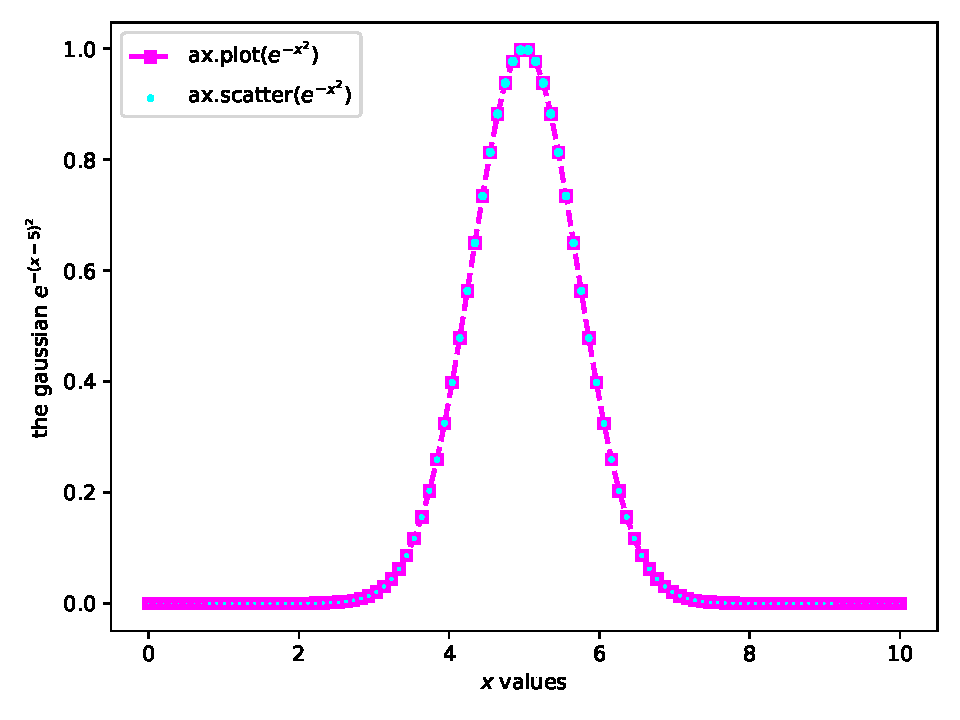
\includegraphics[width=0.5\linewidth]{gaussian.pdf}
\end{center}
Notice that we can control which objects are drawn on top of which using the \ls{zorder=} keyword argument and that basic \LaTeX math typesetting is supported, but latex commands beginning with backslash need to be either escaped (i.e., \verb|"$\\frac{}{}$"|) or in raw strings (i.e., \verb|r"$\frac{}{}$"|).

\begin{exercise}
    Write a program, which will, using NumPy and Matplotlib, graph the expressions $y=x$, $y=x^2$ and $y=\sqrt{x}$ from $x=0$ to $x=5$ with different line styles (e.g., full line, dashed, dotted) and user-supplied number of points. Try linear, semilogarithmic and logarithmic axes. Label the axes and the curves.
\end{exercise}

One figure can contain multiple axes created by passing the optional rows and columns arguments to \ls{plt.subplots()}. The multiple axes are created in a regular grid with a specified number of rows and columns. For axes of unequal sizes, we can specify ratios of their widths and heights using \ls{width_ratios} and \ls{height_ratios} (see \ls{gridspec} \footnote{\url{https://matplotlib.org/3.5.0/tutorials/intermediate/gridspec.html}} for more complicated figure layouts). The axes can share the x and y ranges by specifying the boolean keyword arguments \ls{sharex} and \ls{sharey}, respectively, for example
\lstinputlisting[caption=Multiple axes in single figure.]{../example_code/multiple_axes.py}
\begin{center}
    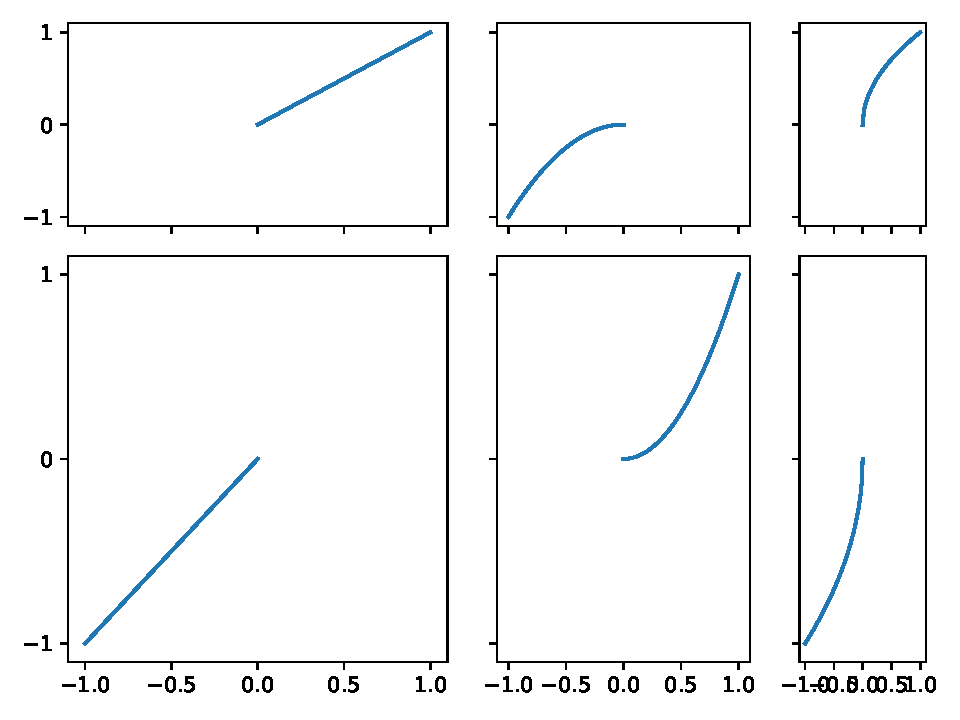
\includegraphics[width=0.5\linewidth]{multiax.pdf}
\end{center}
\begin{exercise}
    \label{ex:peak}
    Write a program that will read the data from "data.txt" which contains three columns of numbers separated by tabs. Let's call these columns frequency, $X$ and $Y$. Plot the frequency dependence of $X$ and $Y$ 
    \begin{enumerate}
        \item in the same axes ($X$ full line, $Y$ dashed line)
        \item in separate axes in the same figure sharing x and y range
    \end{enumerate}
    Plot also $X$ vs. $Y$ in a seprate plot. Label the axes appropriately.
\end{exercise}
\begin{syntax}[Writing modules.]
    Any python file can be imported by any other python file as a module using the \ls{import} keyword, the name of the module is the name of the file (without the .py ending). When \ls{import}ed, the file is first executed, i.e., any code that sits outside of function definitions will run, for example, take two files in the same directory

    \verb|module.py|:
    \begin{lstlisting}
        def my_module_function(x):
            return 1 + x

        print("Hello modules!")
    \end{lstlisting}

    \verb|module_user.py|:
    \begin{lstlisting}
        import module as m
        print(m.my_module_function(1))
    \end{lstlisting}

    Upon running \verb|module_user.py|, "Hello modules!" will be printed. This is usually not desirable. To prevent any code from running when imported and only allow it to run when the file is run directly we can do
\begin{lstlisting}
    if __name__ == '__main__':
        print("Hello modules.")
\end{lstlisting}
    Here, \ls{__name__} is a special variable defined by Python itself that contains the name of the module associated with the current file. Its value is \ls{'__main__'} if and only if it was directly.

    To import a file as a module Python must be able to find it. By default, Python looks in the current working directory \ls{os.getcwd()} and in the directories listed in the list \ls{sys.path} in the package \ls{sys}. If we want to load a package from somewhere else we can simply \ls{sys.path.append()} its directory to the path variable.
\end{syntax}
\begin{exercise}
    \label{ex:peaks}
    Find the maximum and the minimum of the absolute value $R = \sqrt{X^2 + Y^2}$, and indicate their positions using vertical lines in the graph of frequency dependence of $X$ and $Y$ from the previous exercise. Estimate the full-width-at-half-maximum (FWHM) of the peak and the quality factor $f_0$/FWHM, where $f_0$ is the frequency of the maximum response. 
    
    \emph{Hint:} \ls{np.argmin, np.argmax}, \ls{ax.axvline, ax.axhline}
\end{exercise}
\begin{exercise}
    \label{ex:peaks-all}
    Process all files from \ls{lots_of_data} directory similarly to Exc.~\ref{ex:peaks}. Plot the FWHM as a function of $f_0$. Use the solution to Exc.~\ref{ex:peaks} as a module.
    
    \emph{Hint:} \ls{glob}
\end{exercise}

Observables that depend on two control variables can be often plotted using heat maps, for which we can use \ls{ax.imshow(arr2D)}, which takes a 2D array of numbers and maps them to a color of a pixel using a colormap\footnote{See \url{https://matplotlib.org/stable/users/explain/colors/colormaps.html} for a full list of colormap names.} Note however, that \ls{imshow()} is primarily used for images, which conventionally start in the upper left corner with left-handed axes. Data typically start in the lower-left corner with right-handed axes. This can be changed changed by specifying \ls{origin='lower'} keyword to \ls{imshow()}. Alternatively, for plotting data which are not on a regular grid we can use \ls{ax.pcolormesh(X, Y, Z)} where \ls{X, Y, Z} are 2D arrays.

For example, to plot a 2D Gaussian with the \ls{'inferno_r'} colormap,
\begin{lstlisting}[caption=Two-dimensional plotting example.]
import numpy as np
import matplotlib.pyplot as plt

#x and y axis
_xs = np.linspace(0, 10, 100)
_ys = np.linspace(0, 10, 100)
#but we need 100 x 100 points for both x and y that sample the 
#the entire interval (0, 10) x (0, 10), this can be done using
#meshgrid
xs, ys = np.meshgrid(_xs, _ys)
zs = np.exp(-(xs - 5)**2 - (ys - 5)**2)

plt.close('all') #closes all figures we have opened so far
fig, ax = plt.subplots()

plot = ax.imshow(zs, cmap='inferno_r', origin='lower')
#similar
#plot = ax.pcolormesh(xs, ys, zs, cmap='inferno_r') 
cbar = fig.colorbar(plot) #the color axis scaling
cbar.set_label('$z$')
ax.set_xlabel('$x$')
ax.set_ylabel('$y$')
\end{lstlisting}
\begin{center}
    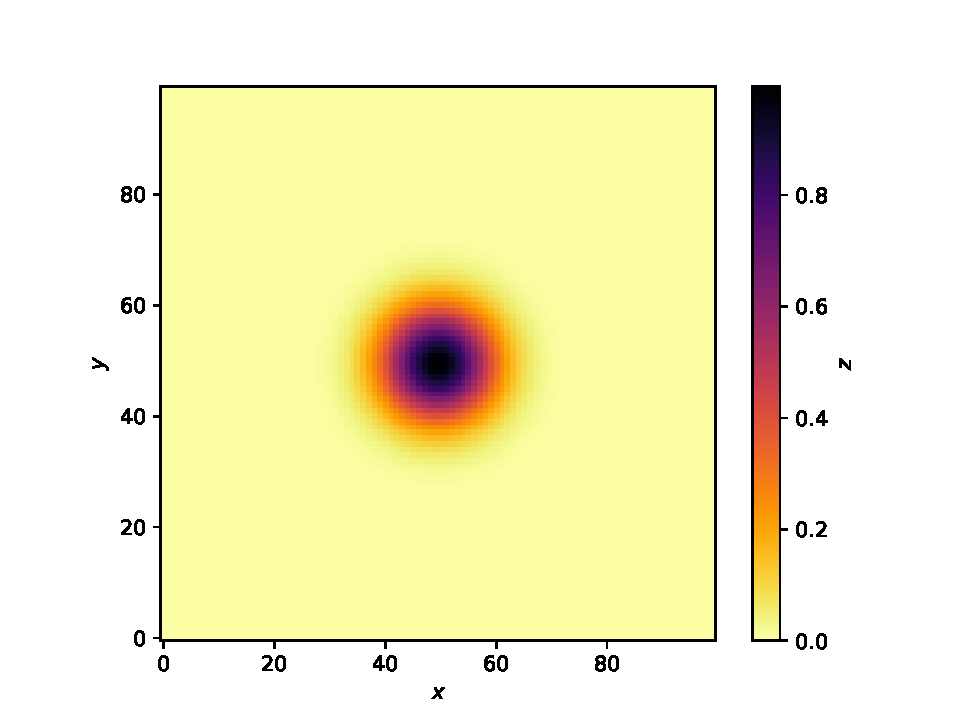
\includegraphics[width=0.5\linewidth]{gaussian_2D.pdf}
\end{center}
\begin{exercise}
    Plot the Mandelbrot set with configurable range and resolution.

    \emph{Hint:} The Mandelbrot set is a set of complex numbers $c$ for which the series $z_{n+1} = z_n^2 + c,\; z_0 = 0$ does not diverge. If $z_n \geq 2$ for any $n$ the series will diverge. As a convergence criterium we can use that $z_n < 2\; \forall n < N_\mathrm{max}$ ($N_\mathrm{max} = 100$, for example). Plot the set using \ls{plt.imshow(c)} where \ls{c[i,j]} is the number of interactions needed to exceed $z_n = 2$ (or $N_\mathrm{max}$). The entire set is contained in the rectangle with lower-left corner $-2-i$ and upper-right corner $1+i$ in the complex plane.
\end{exercise}

\subsubsection{Review of basic plotting commands}
Assuming that the figure and axes were created as \ls{fig, ax = plt.subplots()}, the basic commands for manipulating the plot are

\begin{tabular}{p{40mm}p{100mm}}
     \ls{ax.xlabel("the x-label"), ax.ylabel("the y-label")} & sets the axis labels \\
     \ls{ax.set_xlim(xmin, xmax), ax.set_ylim(ymin, ymax)} & sets the axes limits, xmin, xmax etc. can also be used as keywords \\
     \ls{ax.set_aspect('equal')} & sets the aspect ratio of the axes to be equal, useful when both axes contain qualitatively similar data\\
     \ls{ax.legend(loc=location)} & shows the legend at locatoin \ls{location} $\in$ \ls{"upper|lower left|right"} or \ls{"best"} \\
     \ls{fig.tight_layout()} & adjust the axes size to fit all labels and reduces whitespace\\
     \ls{fig.supxlabel('xlabel'), fig.supylabel('ylabel')} & sets the common figure-wide axis labels for multi-axis figures\\
     \ls{fig.colorbar()} & creates a colorbar in the figure\\
     \ls{plt.close('all')} & closes all open figures
\end{tabular}

\newpage
\section{Least squares fitting and interpolation}
Given data represented by a set of points $[(x_i, y_i)]$, where $x_i$ is the control variable and $y_i$ is the observable (e.g., I control the current through a resistor and observe the voltage), the least-squares fit to a function $f(x; p_1, p_2, ... p_n)$ minimizes the sum of squared residuals, i.e.,
\begin{equation}
    R^2 = \sum_i \left|f(x_i, \{p\}) - y_i\right|^2.
\end{equation}
The result of the fit is a set of parameters $p_1, p_2, p_3, ...$ which minimize $R^2$. Depending on how the function $f$ depends on the parameters $p_k$ we talk about \emph{linear} or \emph{non-linear} fitting. The important difference is the dependence on the parameters $p$, not on the control variable $x$. 

% \subsection{Linear Regression}
% TODO

\subsection{Polynomial fitting.}
Fitting a polynomial in $x$ where the fit parameters are the coefficients of the polynomial is a very common example of linear fitting. Interface for using polynomials is contained in \ls{np.polynomial} submodule in the \ls{Polynomial} class, which provides a 

\lstinputlisting[caption=Polynomial fitting]{../example_code/polynomial_fitting_example.py}
\begin{center}
    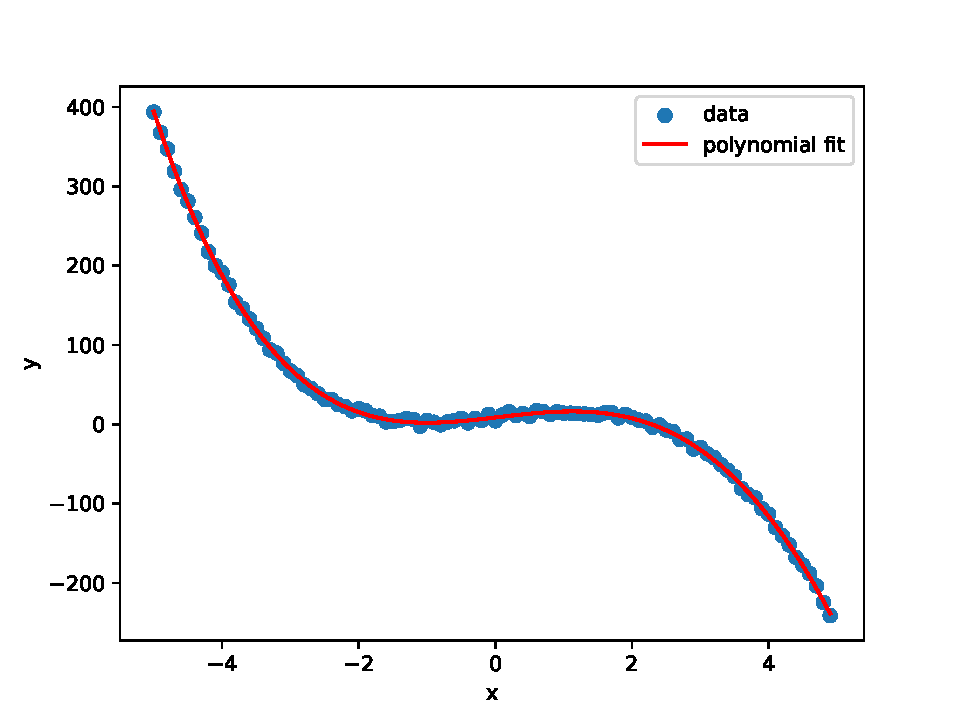
\includegraphics[width=0.5\linewidth]{polynomial_fit.pdf}
\end{center}

\begin{exercise}
    Remove the background from the peaks in exercise~\ref{ex:peaks} using a polynomial fit.

    \emph{Hint}: \ls{np.polynomial.Polynomial.fit()} and boolean arrays
\end{exercise}

\subsection{Non-linear curve fitting}
When the fitting function depends nonlinearly on the fit parameters we need to use nonlinear fitting, several libraries exist for this task, and for basic fitting, we can use \ls{scipy.optimize} submodule of \ls{scipy}.

To fit a given function to data we can use \ls{scipy.optimize.curve_fit}, e.g.,
\lstinputlisting[caption=Nonlinear curve fitting., label=lst:curve-fit]{../example_code/curve_fit_example.py}
\begin{center}
    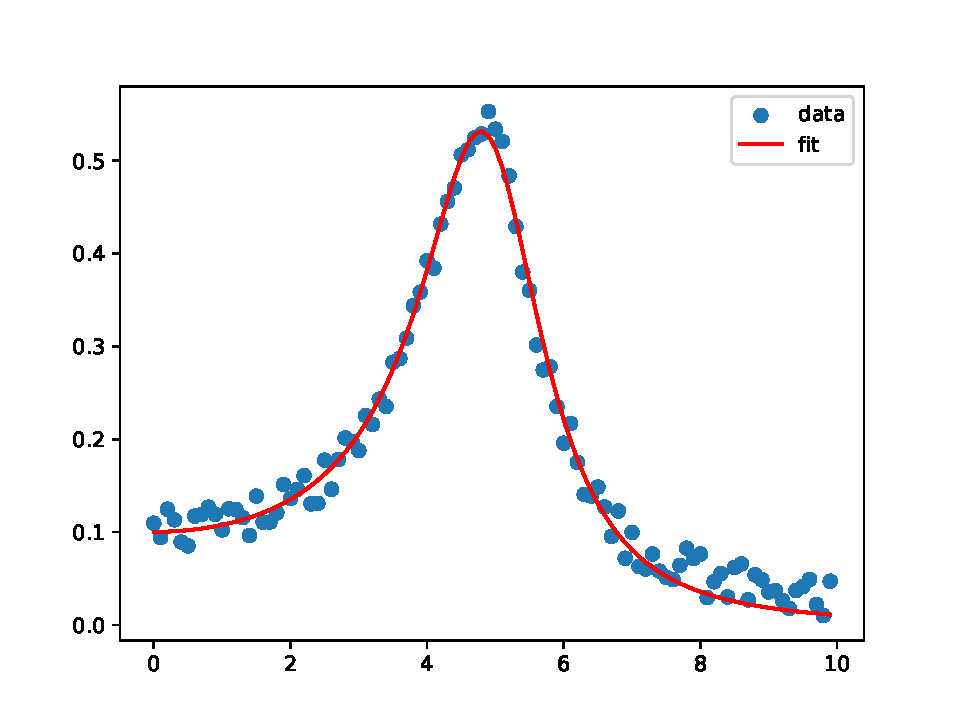
\includegraphics[width=0.5\linewidth]{curve_fit.pdf}
\end{center}

Unlike linear least squares, non-linear curve fitting is iterative and stops once the parameters converge. The fit may never converge for certain problems, therefore, once a configured maximum number of iterations is exceeded the fitting routines \emph{raise an exception} (See \ref{syn:exceptions}) which will crash the program if not handled.

We can use \ls{scipy.optimize.minimize()} for more general optimisation problems. \ls{minimize()} takes a single \textbf{scalar} function and an initial guess for the optimal parameters. For example, to find a minimum of a parabola,
\lstinputlisting[caption=Minimization of a scalar function of multiple parameters.]{../example_code/minimize.py}
\begin{center}
    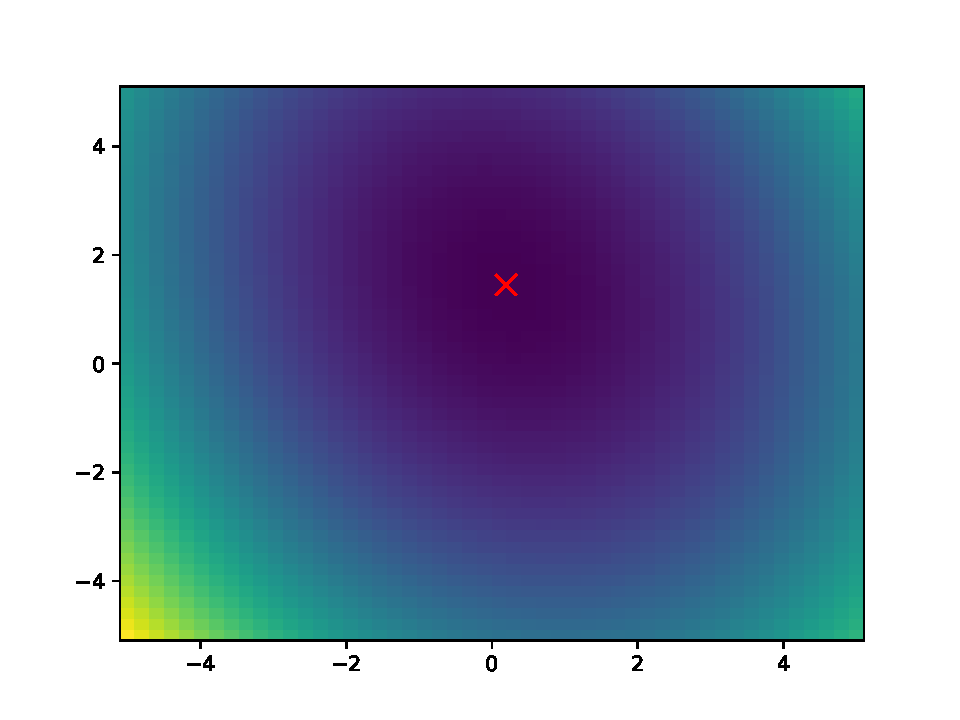
\includegraphics[width=0.5\linewidth]{parabola-minimize.pdf}
\end{center}

\paragraph{Parameter error estimation} The fitting function \ls{curve_fit} returns two values -- the array of the parameters we are interested in and the covariance matrix of the parameters, i.e., $\mathrm{cov}(p_i, p_j) = \langle(p_i - \bar p_i)(p_j - \bar p_j)\rangle$. The diagonal values of the covariance matrix can be used as an estimate of the uncertainties of the fit parameters, i.e.,
\begin{lstlisting}
    #assuming that f is def'ed as f(x, p1, p2)
    p, cov = curve_fit(f, x, y)
    print(f"p1 = {p[0]} +/- {np.sqrt(cov[0,0])}
\end{lstlisting}

The covariance matrix is calculated from the \textit{residuals} $r_i = y_i - f(x_i, \{p_j\})$, where $p_j$ are the optimized parameters as ($\mathbf{r}$ is a vector with elements $r_i$; $i=1\dots N$, $j=1\dots M$) as a scaled inverse of the Hessian matrix $H$ of the objective function $\chi^2 = \sum r_i^2$\footnote{The calculation is slightly more complicated, but similar, when the data points have different weights, see documentation \url{https://docs.scipy.org/doc/scipy/reference/generated/scipy.optimize.curve_fit.html}}
\begin{equation}
    \mathrm{cov}(p_i, p_j) = \frac{1}{N-M}
    \begin{pmatrix}
        \frac{\partial \chi^2}{\partial p_1 \partial p_1} & \frac{\partial \chi^2}{\partial p_1 \partial p_2} & \dots \\
        \frac{\partial \chi^2}{\partial p_1 \partial p_1} & \frac{\partial \chi^2}{\partial p_2 \partial p_2} & \dots\\
        \vdots & \vdots & \ddots
    \end{pmatrix}^{-1},
\end{equation}
where $N$ is the number of data points and $M$ is the number of parameters. Note that usually, we are interested only in the diagonal for the direct error estimate of the fit parameters, however, if, for example, the studied quantity is a sum of two fit parameters $z = A + B$, then the variance of $z$
\begin{equation}
    \mathrm{var} z = \langle (A + B - \bar A - \bar B)^2 \rangle = \langle (A - \bar A)^2 \rangle + \langle (B - \bar B)^2 \rangle + 2\langle (A - \bar A) (B - \bar B) \rangle = \mathrm{var} A + \mathrm{var} B + 2\mathrm{cov}(A, B),
\end{equation}
and the off-diagonal terms of the covariance matrix must be used.

However, the error estimates calculated using the covariance matrix can often be underestimated since the above method is valid only when the model function $f$ is correct and the data truly have the form $y_i = f(x_i, p) + e_i$ where data errors $e_i$ have zero mean and a normal distribution. A more robust, but also more computationally demanding, method of estimating parameter errors is \textbf{bootstrap}, where, for several repetitions, we create a random selection of data (of the same length), perform the fit on each created set and calculate mean and standard deviation (and in principle covariance) on the resulting set of fit parameters, an example implementation is shown in Lst.~\ref{lst:bootstrap}

\lstinputlisting[firstline=24, caption=Estimating fit parameter errors using bootstrap. The data $(x_i\, y_i)$ are created in the same way as in Lst.~\ref{lst:curve-fit}., label=lst:bootstrap]{../example_code/bootstrap_curve_fit_example.py}

\begin{syntax}[Exceptions and error handling]
    \label{syn:exceptions}
    Exceptions are a mechanism used by Python to signal errors or other events which need to be handled by your code. If a \emph{raised} exception is not \emph{caught} the program crashes. To handle exceptions we use the \ls{try}, \ls{except}, and \ls{finally} blocks. We can raise an exception using \ls{raise}. Note that exceptions do not always have to indicate an error, for example, a \ls{for} loop is terminated using a \ls{StopIteration} exception.

    Example of catching and raising exceptions and using the \ls{finally} block.
\begin{lstlisting}

def faulty_function():
    raise ValueError("blergh!")

xs = [-2, -1, 0, 1, 2]
one_over_xs = []
try:
    for x in xs:
        try:
            one_over_xs.append(1/x)
            if x > 1:
                faulty_function()
        except ZeroDivisionError:
            print("Can't divide by zero!")
        except:
            print("something else went wrong")
            raise #propagate the exception further up
finally:
    print("I will always run")

# unless the exception that is raised on line 8 and then sent forward on line 13 isn't
# handled, this line will not run
print(one_over_xs)
\end{lstlisting}
    Notice a few things:
    
    \textbf{\ls{except}} Can catch either a specific type of exception or any type (if the exception type is not specified).
    
    \textbf{\ls{finally} block always runs}, regardless of whether an exception occurred inside the \ls{try} block and is generally meant for proper cleanup (e.g., open files)
        
    \textbf{\ls{try} blocks can be nested}: When an exception is raised, the inner-most \ls{try-except} block tries to handle it. If a suitable \ls{except} is not found or the exception is re-\ls{raise}d, the next enclosing \ls{try-except} block tries to handle it and so on. If the exception gets out of all nested enclosing \ls{try-except} blocks without being handled, the program crashes.
    
    \textbf{\ls{raise} can be used anywhere}, e.g., in functions which do not contain \ls{try}. It is up to the calling code to decide what to do with exceptions
\end{syntax}

\begin{exercise}
    \label{ex:peak-fits}
    Fit the absolute value $r(f) = \sqrt{x^2 + y^2}$ of the response in exercise~\ref{ex:peaks} to the response of a linear harmonic oscillator plus a polynomial background (polynomial degree 3) and plot the results similarly to exercise~\ref{ex:peaks}. Use the simple estimation from exercise~\ref{ex:peak} as initial estimates of the fit parameters. Use the solution to exercise~\ref{ex:peak} as a module.

    Bonus exercise: make the background polynomial degree adjustable

    The complex amplitude of the response of a linear harmonic oscillator to force $F$ is (see Appendix.~\ref{sec:lho})
    \begin{equation}
        x(\omega) = \frac{F/m}{\omega_0^2 - \omega^2 + i\omega\gamma},
    \end{equation}
    where $\omega_0$ is the (angular) resonance frequency, $\omega$ is the frequency of the force $F$, $m$ is the oscillator mass and $\gamma$ is damping.
\end{exercise}
\begin{exercise}
    Estimate the errors of fitting parameters obtained in exercise~\ref{ex:peak-fits} using bootstrap.
\end{exercise}

% lmfit

\begin{syntax}[Object-oriented programming]
    (OOP) is a programming technique for associating data with functions and separating implementation details of partial problems from the rest of the code. If used correctly, it can help with writing easy-to-read, extensible and reusable code.

    In OOP language, objects are instances of classes. Everything in Python is an object. For example, the number 5 is the instance of a class \ls{int}. In modern Python (i.e., version 3 and higher) the concepts type and class have the same meaning. The built-in function \ls{type()} returns the object's class (or type), e.g.,
\begin{lstlisting}
    >>> type(2)
    <class 'int'>
\end{lstlisting}

    To create new classes we use the \ls{class} keyword, e.g., to create a class that represents differences
\begin{lstlisting}
    class Difference:
        def __init__(self, x, y):
            self.x = x
            self.y = y
            
        def __str__(self):
            return f"{self.x} - {self.y}"
        
        def value(self):
            return self.x - self.y
\end{lstlisting}
    Functions defined inside classes are called \textbf{methods}. The first argument, conventionally called \ls{self}, refers to the object that is calling the method. \ls{__init__} is a special method that creates the object, \ls{__str__} is a special function that should create a readable textual representation of the object (used with \ls{print}).

    Using classes and objects is straightforward, e.g.
\begin{lstlisting}
    d1 = Difference(3, 5) #__self__() is called with x=3, y=5 and self refers to d1
    d2 = Difference(30, 50) 

    print(d1.value()) # -2
    print(d2) # "30 - 50"
\end{lstlisting}

    Several other special method names exist (see \url{https://docs.python.org/3/reference/datamodel.html#emulating-numeric-types} for more), e.g. \ls{__add__(self, other)} which is called for \ls{x + y} with \ls{x} being \ls{self} and \ls{y} being \ls{other}. Similarly there are \ls{__sub__}, \ls{__mul__} and \ls{__truediv__} for \ls{-, *, /}, respectively.

\begin{exercise}
    Implement a \ls{Fraction} class that represents a fraction that is initialized by two numbers -- numerator and denominator. The class should support basic arithmetic (\ls{+,-,*,/}) with numbers and other \ls{Fraction}s
\end{exercise}

\end{syntax}

\newpage
\section{Digital signal processing}
\subsection{Digital representation of a continuous signal}
Assume a signal $y(t)$ (e.g., a voltage) which varies continuously in time. To store and process this signal on a computer we measure it at a set of time instants $t_i$ yielding values of the signal $y_i$, resulting in the discrete representation of the signal as a series of pairs $(t_i, y_i)$. The signal is uniformly sampled if $t_i = i\Delta t$, where $\Delta t$ is the \textbf{sampling period} and $f_s = 1/\Delta t$ is the \textbf{sampling frequency}.

Any information about the original signal $y(t)$ that varies in time faster than $\Delta t$ is lost. However, if $y(t)$ oscillates at a frequency $f$ it is insufficient to have $f_s \geq f$. Signal frequencies $f > f_s/2$ will appear shifted to $f - f_s/2$, see the output of Lst.~\ref{ls:label}. The sampled signal contains fictitious frequencies which are not present in the original signal. 

This distortion of called \textbf{aliasing} and the \emph{Nyquist theorem} states that in order to avoid aliasing, the highest frequency contained in the signal $f$ must not be higher than one half of the sampling frequency $f_s/2$, which is called the \textbf{Nyquist frequency} 
\begin{equation}
    \label{eq:nqyust}
    f_N = f_s/2.
\end{equation}

\lstinputlisting[caption=Effect of sampling rate, label=ls:label]{../example_code/sampling.py}
\begin{center}
    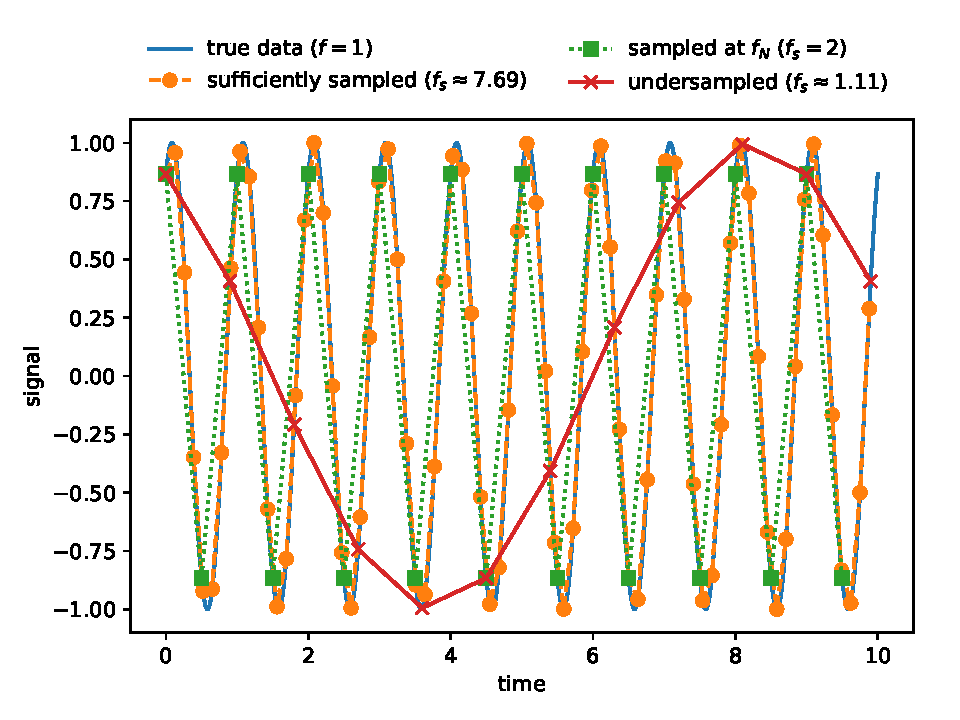
\includegraphics[width=0.75\linewidth]{sampling.pdf}
\end{center}

\subsection{Spectral analysis}
Any periodic signal $y(t)$ (which can be complex) with a period $T$, i.e., $y(t + T) = y(t)$, can be represented as a sum of sine and cosine terms oscillating at angular frequencies $2\pi n/T$ where $n$ is an integer,
\begin{equation}
    y(t) = \frac{1}{T} \sum_{k=0}^{\infty} A'_k\sin\left(\frac{2\pi k}{T}t\right) + B'_k\cos\left(\frac{2\pi k}{T}t\right),
\end{equation}
which is called the \textbf{Fourier series}. Equivalently, the Fourier series can be expressed using complex exponentials
\begin{equation}
    y(t) = \frac{1}{T} \sum_{k=-\infty}^\infty A_k e^{2\pi ikt/T},
\end{equation}
where for a real signal $y$ the positive and negative terms are complex conjugate, $A_k = A_{-k}^*$ (the $1/T$ factor and sign inside the exponential function are conventional).

Fourier coefficients $A_k$ can be calculated as
\begin{equation}
    A_k = \int_0^T y(t) e^{-2\pi ikt/T} \mathrm{d}t
\end{equation}

For example, consider the directly-calculated Fourier series in Lst.~\ref{lst:fourier-square-pulse}
\lstinputlisting[label=lst:fourier-square-pulse, caption=Fourier series of a square pulse.]{../example_code/fourier_series_square_wave.py}
\begin{center}
    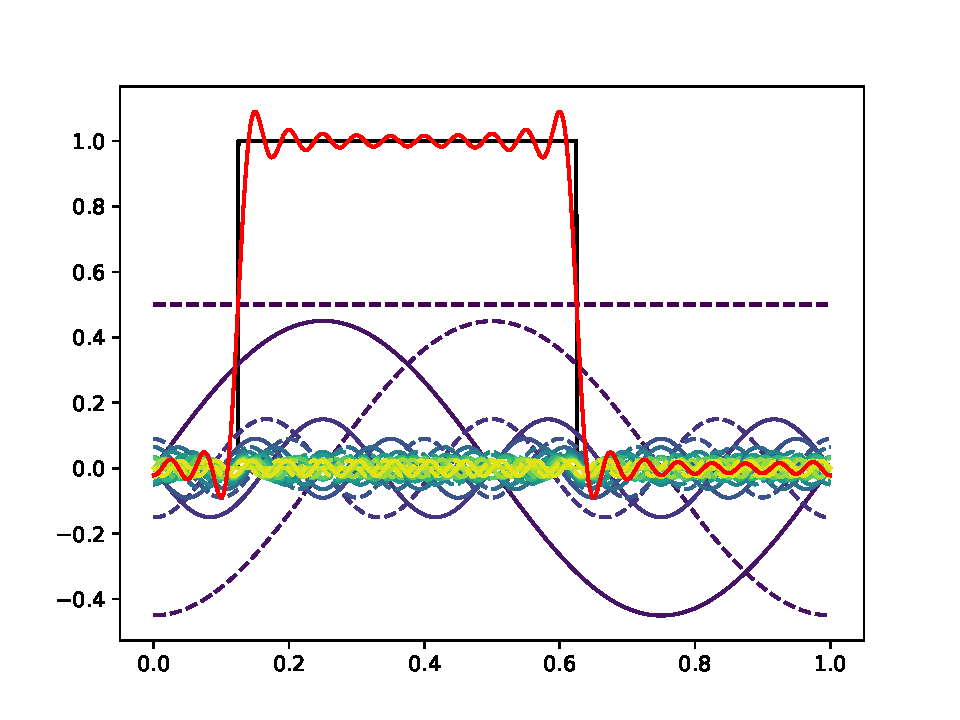
\includegraphics[width=0.5\linewidth]{fourier_series_square_pulse.pdf}
\end{center}

These definitions can be extended to aperiodic signals (which can be imagined as signals with infinitely long periods) which yields the \textbf{Fouerier transform}
\begin{equation}
    \tilde y(\omega) = \int_{-\infty}^\infty y(t)e^{-i\omega t} \mathrm{d}t,
\end{equation}
and the \textbf{inverse Fourier transform}
\begin{equation}
    y(t) = \frac{1}{2\pi}\int_{-\infty}^\infty \tilde y (\omega)e^{i\omega t}\mathrm{d}\omega
\end{equation}

The absolute value of the Fourier coefficients $|A|$ is the amplitude of the signal's oscillation at a given frequency and their complex phase is the phase rotation of the sine and cosine terms. For the Fourier transform, since the frequency now varies continuously, the $|\tilde y|$ has a meaning of \emph{density} (called spectral density). In analogy with electrical power $P = V^2/R$ needed to generate voltage $V$ across a resistor $R$, $|\tilde y|^2$ is called the \emph{power spectral density}, i.e., $\int_{\omega_0}^{\omega_1} |\tilde y (\omega)|^2\mathrm{d}\omega$ is the power of the signal in the frequency band $(\omega_0, \omega_1)$.

For digital signals, we talk about \emph{discrete} Fourier transforms. For uniformly sampled signals, $t_n = n\Delta t$ these are in SciPy defined as (in the submodule \ls{scipy.fft})
\begin{equation}
    \tilde y[k] = \sum_{n=0}^{N-1}y[n]e^{-2\pi i kn/N},
\end{equation}
where $y[n]$ is the value of the signal $y$ measured at time $t_n = n\Delta t$ and $N$ is the total number of samples. The dimensionless integer frequencies $k$ run from 0 to $N-1$ -- that is, the fourier transform has the same length as the original signal. 

The inverse discrete Fourier transform is defined similarly,
\begin{equation}
    y[n] = \frac{1}{N}\sum_{k=0}^{N-1}\tilde y[k]e^{+2\pi i kn/N}.
\end{equation}

The integer frequency indices $k$ represent frequencies $f'_k = k/N$ for $k=0\dots N/2$ and $f'_k = -k/N$ for $k=N/2\dots N-1$. To get the actual frequencies we only need to scale $f'_k$ with the actual sampling frequency $1/\Delta t$. Notice that the definitions of the discrete Fourier transform and its inverse do not depend on the sampling rate, only on the fact that the signal is sampled uniformly.

Fourier transforms are implemented in NumPy and SciPy using the \textbf{Fast Fourier Transform -- FFT} algorithm\footnote{FFT is one of the most important algorithms that the entire digital world depends on -- e.g., sound and video encoding and wireless communication rely on it heavily.} in the \ls{scipy.fft} submodule. Fourier transform is calculated using \ls{scipy.fft.fft()} and the actual frequencies can be calculated using a helper function \ls{scipy.fft.fftfreq()}. Both \ls{fft} and \ls{fftfreq} return positive and negative frequencies. For real signals, the negative frequencies do not provide any extra information therefore we can use \ls{scipy.fft.rfft()} and \ls{rfftfreq()} which return only positive frequencies (i.e., the result is half the length of the original signal). If we are only interested in the power spectral density, there is \ls{scipy.signal.periodogram()} which also calculates the frequencies. By default, for real signals, \ls{periodogram} returns only the positive frequencies and both positive and negative frequencies for complex signals. See Lst.~\ref{lst:fouriers} for example usage and Lst.~\ref{lst:fft-square-wave} for a version of the program in Lst.~\ref{lst:fourier-square-pulse} but using FFT rather than manual calculation of the coefficients

\lstinputlisting[caption=Calculation of Fourier transform and power spectral density., label=lst:fouriers]{../example_code/fouriers.py}
\begin{center}
    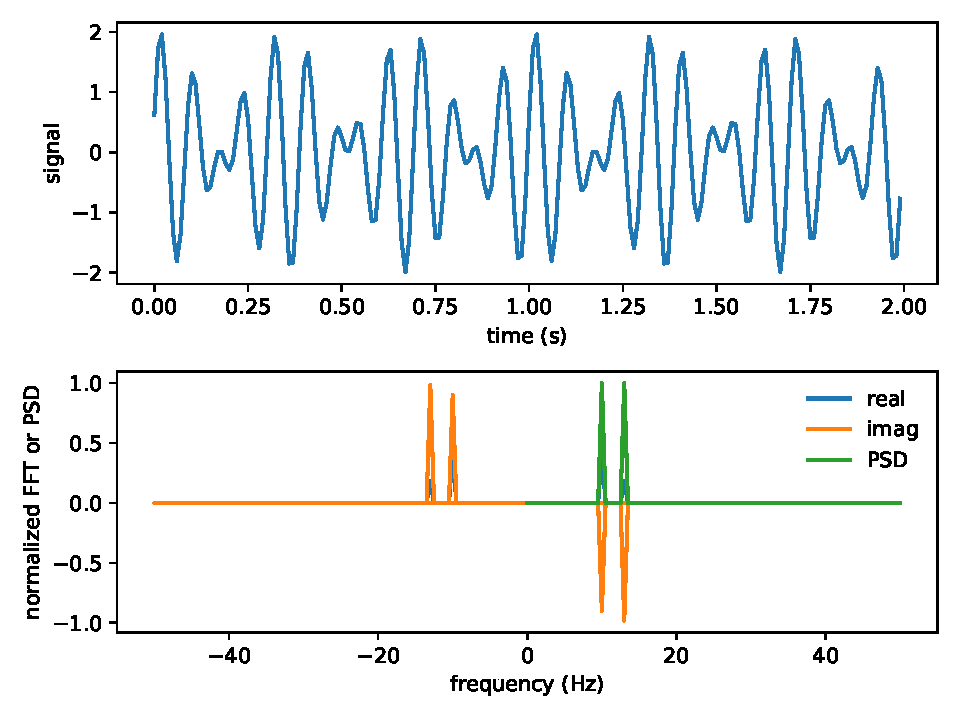
\includegraphics[width=0.5\linewidth]{fouriers.pdf}
\end{center}

\lstinputlisting[label=lst:fft-square-wave, caption=Fourier coefficient of a square wave\, calculated using FFT]{../example_code/fourier_series_square_wave_fft.py}

One particularly important Fourier transform is that of the exponentially deacying oscillation, i.e.
\begin{equation}
    s(t) = e^{-t/\tau}\sin(2\pi f t),
\end{equation}
which yields the complex lorentzian which is the response of the linear harmonic oscillator, see Sec.~\ref{sec:lho}. The decaying oscillation is, of course, the motion of the damped unforced linear harmonic oscillator. Example:
\lstinputlisting{../example_code/decaying_exponential.py}
\begin{center}
    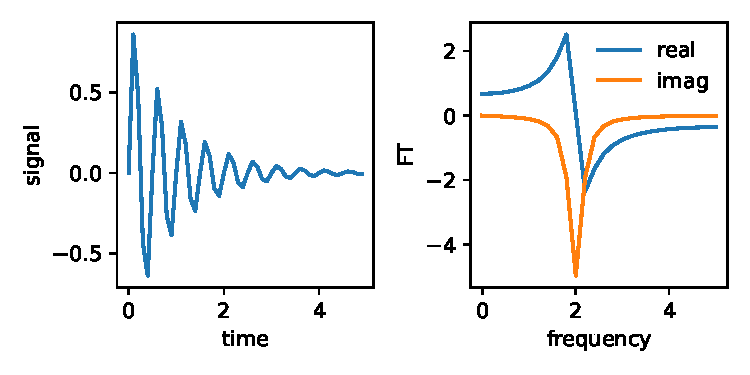
\includegraphics{decaying_exponential.pdf}
\end{center}

\begin{syntax}[Storing data and metadata in numpy binary files.]
    \label{syn:npy}
    So far, when loading data from a disk, we encountered only simple human-readable text files. This is a very limiting way to store data: the data have to have the form of a rectangular table, the files take up more space than necessary (e.g., text \ls{1.234567890} requires 11 bytes of memory but a \ls{float} representing the same number only needs 8), and it is cumbersome to store metadata.

    Many file formats address these issues (e.g., HDF5 is popular). Here we will use a solution that does not require any further external libraries -- storing dictionaries in compressed binary \ls{.npy} files, e.g. saving
\begin{lstlisting}
    raw_data = np.linspace(0, 1, 50)
    my_data = {
        'date of measurement': '20241224',
        'was Mercury in retrograde': False,
        'data': raw_data
    }
    np.save("my_data.npy", my_data)
\end{lstlisting}
    and loading
\begin{lstlisting}
    my_data = np.load("my_data.npy", allow_pickle=True).item()
    print(my_data['date of measurement'])
    print(my_data['data'])
\end{lstlisting}

    \textbf{Pickling} is a Python term for storing almost any Python object on disk as binary data. Loading a pickled object can in, some circumstances, be a security risk (i.e., avoid reading pickled data you downloaded from weird places on the internet), therefore we have to allow it explicitly. Functions \ls{np.load} and \ls{np.save} are working with arrays, therefore \ls{np.load()} returns an array of length 1 where our dictionary is the only element. The method \ls{array.item()} returns \ls{array[0]} if \ls{array} is length 1 or raises a \ls{ValueError} exception otherwise. Its purpose is to semantically indicate that we expect the array to only have one element and if it does not, something is wrong.
    
    \begin{exercise}
    Read data from the directory \ls{timeseries_data} and plot the time-dependence of the approximate mean temperature during the measurement. Read the files using \ls{d = np.load(filename, allow_pickle=True).item()}. The temperature at the beginning and end of the measurement period is \ls{d['Ti']} and \ls{d['Tf']}, respectively.
    
    \emph{Hint:} To get the timestamp (number of seconds since 00:00 1.1.1970) you can use \ls{time.mktime(time.strptime(fn, 'DM_\%Y\%m\%d-\%H\%M\%S.npy'))}, with \ls{fn} the filename.
\end{exercise}
\end{syntax}

\begin{exercise}
    Plot the time series and spectral density of the pulse used to drive the resonance in the \ls{data/timeseries_data} binary data files (see Storing and loading binary files \ref{syn:npy}) using \ls{scipy.signal.periodogram} and using the (r)FFT functions from \ls{scipy.fft}. The pulse can be loaded as \ls{d['pulse']}, the number of points can be obtained as \ls{d['samples']} (same as \ls{len(d['pulse'])} and the sampling rate as \ls{d['samples']}. Plot only one file (the pulse is the same for all).
\end{exercise}

\begin{exercise}
    Plot the time series (as a function of actual time) of the resonator response (\ls{d['timeseries']}) and its frequency dependence (both real and imaginary components) for the file corresponding lowest temperature in the \ls{timeseries_data} directory. Calculate the frequency response as a ratio of the Fourier transforms of the resonator response and the driving pulse. Plot only frequencies $|f| < 3000$, the resonance is in the range of approximately 2000 - 2400 Hz.
\end{exercise}

\begin{exercise}
    \label{ex:response-heat-map}
    Plot the magnitude (i.e., absolute value) of the response of the resonator $r$ as a 2D heat map plot as a function of both frequency and temperature (i.e., each line in the 2D plot should be a single spectrum corresponding to a single temperature).
\end{exercise}

\begin{exercise}
    As exercise~\ref{ex:response-heat-map}, but average together all spectra closer than 50 mK in temperature (this smoothing technique is called moving average or adjacent averaging).
\end{exercise}

\paragraph{Amplitude, power, and decibel}

In signal processing we often talk about attenuation or gain (or amplification) of a system, e.g., wiring, amplifiers or attenuators. Gain is defined as the ratio of output to input signal and is often measured in decibels defined as
\begin{equation}
    g = 10\log_{10}\frac{s_\mathrm{out}}{s_\mathrm{in}} \mathrm{[dB]}
\end{equation}
or for power, i.e., $s = V^2$,
\begin{equation}
    g = 20\log_{10}\frac{V_\mathrm{out}}{V_\mathrm{in}}
\end{equation}

For "absolute" quantities measured in dB (e.g., sound amplitude is common) the measurement is defined with respect to some agreeed upon reference value. For sound the acoustic power (i.e., pressuer squared) is measured relative to 20 \textmu P in air. In electronics, particularly radiofrequency (RF) engineering, a common unit is dBm, where 0 dBm is equivalent to 1 mW of power, i.e., for a 50 \textohm load about 0.224 V$_\mathrm{RMS}$.

For amplitudes, doubling the signal corresponds to +3 dB and halving the signal to -3 dB and for power it is +6 dB and -6 dB.

\subsection{Filters}

Filtering is a procedure by which we remove certain frequency ranges from the input signal. These procedures are general, but the simplest ones are based on the analogy with simple electronic RC filters, see Fig.~\ref{fig:RC-lowpass}. Depending on the arrangement of the rezistor and capacitor we create a circuit which either attenuates low or high frequences.
\begin{figure}
    \centering
    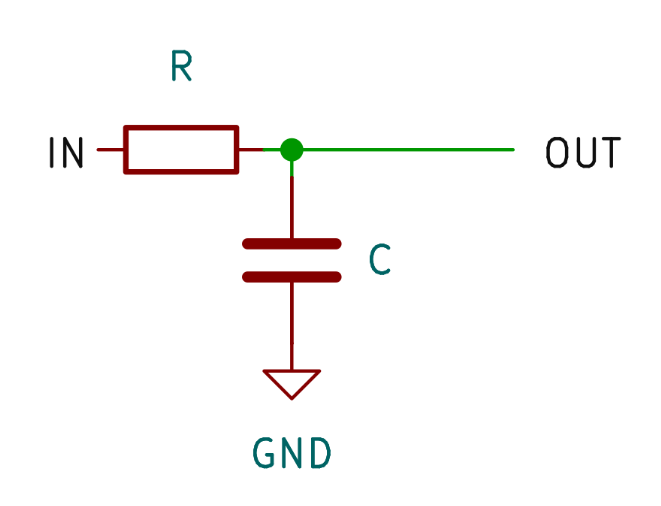
\includegraphics[width=0.49\linewidth]{low-pass-RC.png}%
    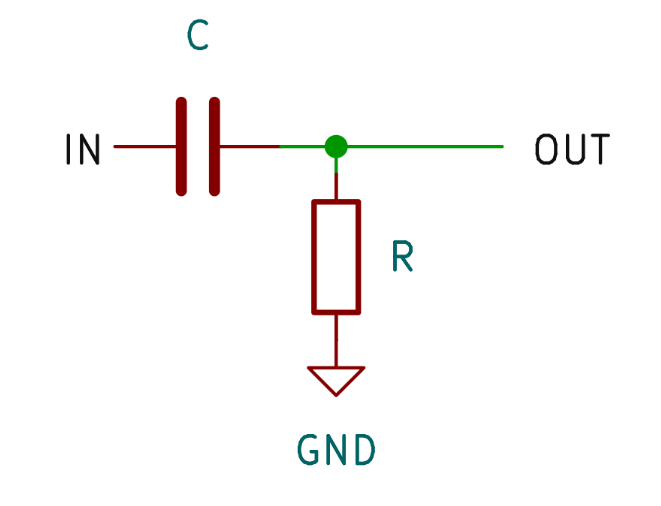
\includegraphics[width=0.49\linewidth]{high-pass-RC.png}%
    \label{fig:RC-lowpass}
    \caption{Low-pass (left) and high-pass (right) RC filter.}
\end{figure}

Using the impedance of a capacitor $Z_C = (i\omega C)^{-1}$ for voltage oscillating at angular frequency $\omega$, we get for the low-pass filter
\begin{equation}
    \frac{V_\mathrm{out}}{V_\mathrm{in}} = \frac{1}{1 + i\omega RC},
\end{equation}
and for the high pass
\begin{equation}
    \frac{V_\mathrm{out}}{V_\mathrm{in}} = \frac{i\omega RC}{1 + i\omega RC}.
\end{equation}
The above expressions are called transfer functions of the filter. Quantity $RC = \tau$ is called the time constant. The corner frequency $f_c = 1/(2\pi\tau)$ is the frequency when the filter starts acting. We can plot the response of the filters with the following code
\lstinputlisting[firstline=4,lastline=12]{../example_code/RC_filters_response.py}
\begin{center}
    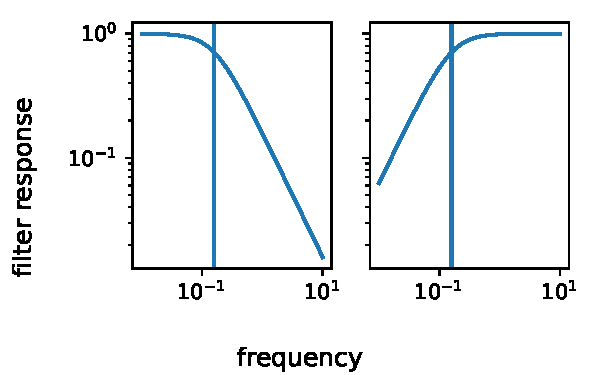
\includegraphics{RC_filters.pdf}
\end{center}
The figure shows the absolute value of the transfer function for the low-pass and high-pass RC filters, respectively. The vertical line is the corner frequency.

Notice that the transfer functions are functions of frequency and the circuits they represent are linear, i.e. they act on each frequency independently. Therefore, if $s(t)$ is out signal and $\hat s(f)$ is its Fourier transform, the Fourier transform of the signal filtered with a tranfer functino $H(f)$ is simply
\begin{equation}
    \hat s'(f) = H(f)\hat s(f),
\end{equation}
i.e., filters in frequency domain simply multiply the spectrum. In time domain $s'(t) = \mathcal{F}^{-1}[H\hat s]$; Fourier transform of a multiplication is a convolution, i.e.
\begin{equation}
    s'(t) = (h*s)(t) \equiv \int_{-\infty}^t s(t')h(t - t')\dd t,
\end{equation}
where $h$ is the inverse Fourier transform of $H$ and is called the convolution kernel. Note that FFT is often the fastest way to calculate a convolution, although we do not have to implement it ourself since there is \ls{scipy.signal.convolve(a, b)}, which calculates the convolution of signals \ls{a} and \ls{b}.

For the low-pass RC filter it can be proven that
\begin{equation}
    h(t) = \left\{\begin{matrix}
        e^{-t/\tau} & \mathrm{for}\; t > 0 \\
        0 & \mathrm{for}\; t < 0
    \end{matrix}\right.
\end{equation}
which can also be easily implemented for streaming data, for which it is often called \emph{exponential smoothing}.

Apart from low-pass and high-pass filters there are also band-pass and band-stop filters. Band-pass only lets through a certain frequency badn and band-stop lets through everything except for a certain frequency band. You can imagine band-pass as a high-pass followed by a low-pass in series and band-stop as a low-pass and high-pass in parallel with corner frequencies given by the pass or stop band. 

The simple RC filters above are so-called first order. The order of the filter indicates how fast it cuts the signal outside of the \emph{pass band} (i.e., the interval of frequencies which the filter lets through). This is often measured in decibels per octave (dB/oct) which indicates by how many decibel is the signal attenuated if its frequency doubles, for a low-pass filter, or halves for high-pass filter, sufficiently far from the corner frequency. Both of the RC filter are 6 dB/oct, since every doubling of frequency remove 6 dB of transmitted power.

Faster filters can be constructed both electronically and digitally, but as you saw in the examples with the step function, sharp cutoff in the spectrum leads to oscillations, which are typically undesirable. The filters that are maximally flat in the pass-band are the Butterowrth filters, named after S. Butterowrth, which have amplitude gain
\begin{equation*}
    G_n(\omega) = \frac{1}{\sqrt{1 + \frac{\omega^{2n}}{\omega_c^{2n}}}},
\end{equation*}
where $\omega_c$ is the corner (angular) frequency. We can construct these filters using \ls{scipy.signal.iirfilter} and apply it to our signal using \ls{scipy.signal.sosfilter}
\lstinputlisting[firstline=7, lastline=25]{../example_code/sig_iirfilter.py}:
\begin{center}
    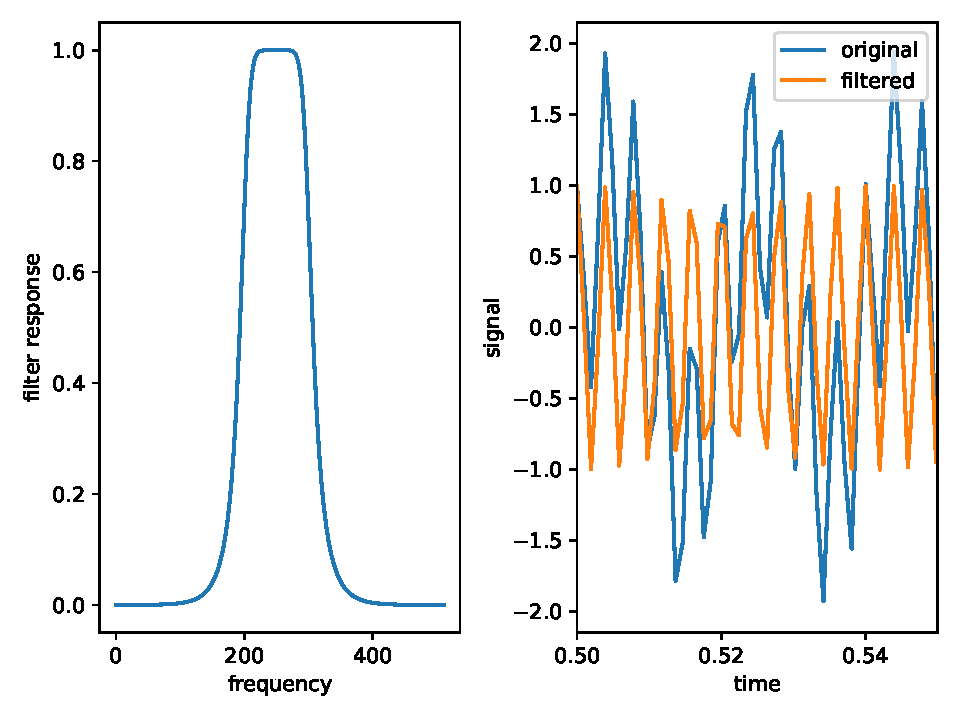
\includegraphics[width=0.5\linewidth]{butter.pdf}
\end{center}

\begin{exercise}
    \label{ex:filter}
    Write a function, which will filter the input signal using
    \begin{enumerate}
        \item low-pass RC filter with adjustable cutoff frequency
        \item high-pass RC filter similarly to 1.
        \item Butterworth band-pass filter constructed using \ls{scipy.signal.iirfilter()} and applied using \ls{scipy.signal.lfilter()}
    \end{enumerate}

    For 1. and 2. plot the the filter transfer function. Test the filtering on the attached \ls{noisy_data.npy} and plot the signal in both the time and frequency domain before and after filtering. For the low-pass filter, filter out everything above 100 Hz. For high-pass, everything below 1000 Hz and for band-pass leave only the range (4310, 4330) Hz.
\end{exercise}

% \subsection{Homodyne and heterodyne detection, signal envelope}
% TODO: mixing, homodyne and heterodyne detection, lock-in amplification

\begin{exercise}
    \label{ex:envelope-direct}
    Demodulate the cleaned-up signal from Exc.~\ref{ex:filter} (using Butterworth band pass filter) on the carrier frequency 4321 Hz (multiply by $e^{i\omega t}$ and low-pass filter) and plot the envelope modulating the carrier wave.
\end{exercise}

\begin{exercise}
    \label{ex:envelope-hilbert}
    Calculate the signal envelope from Exc.~\ref{ex:envelope-direct} using the Hilbert transform.
\end{exercise}

\subsection{Interpolation and smoothing.}

TODO: \ls{scipy.ndimage.gaussian_filter()}, \ls{scipy.signal.savgol_filter()}, \ls{scipy.interpolate.interp1d()}, \ls{scipy.interpolate.UnivariateSpline()}

\newpage
\section{Communication with instruments}
Instrumentation can be connected to a computer through a wide variety of interfaces, including USB, GPIB, RS-232 or Ethernet or emulated serial port over USB. Each of these interfaces require specific OS support, drivers or libraries to use. This was, fortunately, to a large degree solved by the Virtual Instrument Software Architecture (VISA) which abstracts and unifies most of the interfaces into VISA "sessions".

Most of the communication over VISA sessions is text-based. A text command is sent to an instrument, the instrument performs some action and, optionally, replies a text response back. To use VISA we will use the \lstinline|pyvisa| python module. This, however, is only a python interface to the system VISA library. There are several implementations of the VISA library (sometimes called the VISA backend) from multiple vendors, e.g., from National Instruments (NI-VISA, most common) or Keysight companies. We will be using an open-source fully-python VISA backend \lstinline|pyvisa-py|. For our purposes will also need \lstinline|pyserial|. If you want to use USB, Ethernet or GPIB instruments, one of the free-to-download proprietary implementation is probably the best way forward.

In this course we will be using the Raspberry Pi Pico in place of an actual instruments. The Pico is programmed to respond to several commands that roughly follow the SCPI syntax (see Appendix~\ref{sec:pico}). A simple VISA program that communicates with an instrument might look like this
\lstinputlisting{../example_code/visa_intro.py}
On the first line we import the \lstinline|pyvisa| module. Creating new sessions is done via the Resource Manager \lstinline|rm|. In the VISA naming convention instruments are called 'resources' and they are identified by a resource address, which will typically indicate the type of interface used, e.g., addressed that begin with \lstinline|ASRL| are serial instruments, \lstinline|GPIB| and \lstinline|USB| etc.

The resource manager provides the \lstinline|list_resources()| method which returns a list of all available resources. For USB and GPIB these are usually the instruments actually connected to the computer. For serial interface, all available ports might be listed regardless of whether something is connected to them or not.

To start a VISA session, we use the \lstinline|open_resource()| method of the resource manager. In addition, here we specify the read and write termination, which are characters that indicate that the transmission is finished (think of army movies when they say "over" to a walkie-talkie). The new line \ls{'\\n'}, carriage return \ls{'\\r'} and their combination \ls{'\\r\\n'} are common. Our pico expects the commands to be terminated by new line \ls{'\\n'} and terminates its responses with a new line as well. For other instruments, this is something you have to find in the manual, but \ls{'\\n'} is the most common.

The open VISA session is represented by the object \ls{pico} returned by \ls{open_resource()}, whose most important methods are \ls{write()}, \ls{read()} and \ls{query()}, which is simply a write immediately followed by a read.

Most scientific instruments will communicate via text strings which usually adhere to the syntax specified by Standard Commands for Programmable Instruments (SCPI), which tries to define a common syntax for instruments of similar type. SCPI commands typically have the format
\begin{lstlisting}
    :COMMand:SUBCommand:SUBCommand ARG1 ARG2 ...
\end{lstlisting}
where the capitalized substrings can be used as a shorthand. For example, on most digital multimeters (e.g., the venerable Keithley 2000 series), command
\begin{lstlisting}
    :MEAS:VOLT:DC?
\end{lstlisting}
will measure the DC voltage. The question mark at the end indicates that the command returns a value. Instruments that support SCPI in addition support several basic commands such as \ls{*IDN?}, which returns an identification string, \ls{*STB?}, which returns a single byte with various status bits of the instrument or \ls{*RST}, which resets the instrument. At the end, both the VISA session and the resource manager should be properly closed using the \ls{close()} method.

In most cases, nothing other than the resource address is necessary for the \ls{rm.open_resource()} method to successfully open the session. However, especially for some older instruments connected via RS-232, some additional information is often required. Assuming that a device was opened as \ls{dev = rm.open_resource(address)}, before we can start communicating we might need to set the following:
\begin{description}
    \item[baud rate] Number of changes to the communication signal per second (i.e., changes from low to high voltage). Can be set via \ls{dev.baud_rate} to an integer.
    \item[data bits] Number of actual data bits in a single "packet" of data exchanged between the instrument and computer (usually 8). Can be set via \ls{dev.data_bits} to an integer.
    \item[stop bits] The number of bits indicating beginning and end of a character transmitted on serial cable (usually 1). Can be set via \ls{dev.stop_bits} to one of \ls{pyvisa.constants.StopBits.SB} where \ls{SB} is \ls{one}, \ls{one_and_a_half} or \ls{two}.
    \item[parity] A simple check for corrupted transfer. Some instruments send a bit indicating whether the sum of bits in the last character (i.e., its ASCII code) was odd or even. Can be set via \ls{dev.parity} to one of \ls{pyvisa.constants.Parity.P} where \ls{P} is \ls{none} (most common, no parity check), \ls{even} or \ls{odd}.
\end{description}
For example, if we had an instrument on address \ls{COM16} and its manual says that it expects baud rate of 19200, 8 data bits, one stop bit and no parity we could open the communication as
\begin{lstlisting}
    import pyvisa as vi

    rm = vi.ResourceManager()
    dev = rm.open_resource('COM16')
    dev.baud_rate = 19200
    dev.data_bits = 8
    dev.stop_bits = vi.constants.StopBits.one
    dev.parity = vi.constants.Parity.none

    dev.query('*IDN?')
    ...
\end{lstlisting}

\begin{exercise}
    Create a program that automatically finds the pico if it is connected to the computer. Send the \ls{*IDN?} query to every available VISA resource and find the one that responds \ls{'PICO'}. Resources (serial ports) which are not connected to any instrument will raise a timeout exception, which must be handled without crashing the program.
\end{exercise}

\begin{exercise}
    Open the communication to the pico and make the white and blue LEDs flash in a "police car"-like pattern (i.e., two quick flashes of white followed by two quick flashes of blue) on repeat. Use the \ls{:LED n x}, where $n=0\dots 4$ is the LED number and $x$ is either 0 or 1, which turns the LED off or on. Make sure that when your program is killed (either by Ctrl-C or the interrupt button in Spyder) all LEDs are turned off.
\end{exercise}

\begin{exercise}
    Write a program that will indicate the current temperature (obtained using \ls{:READ:T?} command) using the on-board LEDs. Map the range 20-27$^\circ$C to 0 to 5 LEDs ON. If the temperature exceeds 28$^\circ$C, raise a \ls{RuntimeError}, which ends the program. Make sure none of the LEDs stay on when the program ends.
\end{exercise}

\begin{exercise}
    Write a "digital spirit level", i.e., indicate the current tilt along the y-axis (length-wise along the PICO) using the LEDs (you can decide on whatever you think is the best way to use the LEDs). Note that the accelerometer is not soldered to the PCB perfectly level. Assume that when the program is run, the pico is level and use the acceleration vector measured at the beginning as the reference value.
\end{exercise}

\begin{exercise}
    Write an object interface to the pico, which should be initialized using only the resource manager instance and should find the correct address on its own, i.e.,
    \begin{lstlisting}
        import pyvisa as vi

        class Pico:
            def __init__(self, rm):
                ...
            def led(self, led_id, onoff):
                #should raise ValueError if led_id > 4
                ...
            def getT(self):
                ...
            def getP(self):
                ...
            def getACC(self):
                ...
            def getGYR(self):
                ...
            def close(self):
                "Turn off all LEDs and close the session."
                ...
        
        rm = vi.ResourceManager()
        pico = Pico(rm)
        pico.led(2, 1) #turns the middle LED ON
    \end{lstlisting}
\end{exercise}

\subsection{Context Management Protocol}
Particularly with instruments that control actual laboratory hardware, proper shutdown and cleanup, even in the event of a software error, is very important. Imagine an oven, which keeps heating up, or a motor which keeps spinning uncontrollably because of a typo in your program. We saw in Exercises 27 -- 29 that a controlled shutdown can be handled using the \ls{finally} clause after a \ls{try} block. This is suboptimal, because we have to remember to write the \ls{finally} block, which is often does not change much, in every program in which we use a given instrument.

Python has a solution for this, which we already saw, called \emph{context management protocol}, which is what the \ls{with} statement uses. Recall using files,
\begin{lstlisting}
    with open("hello.txt", 'w') as file:
        file.write('Hello Context Management.')
\end{lstlisting}
where the \ls{with} statament makes sure that after we are done using the file it is properly \ls{close()}d

To use the context management with our objects we only need to define two special methods, \ls{__enter__()} and \ls{__exit__()}, which are run at the beginning and end of the with statement. The enter method should return the object we want to use (i.e., file in the above example), often it simply returns \ls{self}. The exit method should do all the necessary cleanup. It takes three additional arguments besides \ls{self} which contain information about whether an exception occurred and what type. Most of the time we can ignore the exceptions and simply let it propagate. If we return \ls{False} from the exit method, the exception is supressed.

Take a simple example. Say we want to have file-like object that can be used with \ls{with} as an ordinary file but the method \ls{write()} also supports NumPy arrays. We could do the following
\lstinputlisting{../example_code/context_management_file.py}
which prints
\begin{verbatim}
    I'm about to open the file.
    Opening file.
    Entering with statement
    Closing.
    The end
\end{verbatim}

Notice that the method \ls{__enter__()} simply returns \ls{self}. This is because the context manager and the object representing the file are the same. In the \ls{__exit__()} method we simply lump together all information about any exception that might have occurred in the \ls{*exc} argument list and ignore them, only doing the necessary cleanup. Not returning anything is equivalent to returning \ls{None}, which is not \ls{False}, so if any exception occurred it will simply continue on its merry way to the nearest \ls{except} clause.

\begin{exercise}
    Extend the Pico class to support the context management protocol.
\end{exercise}

For completeness, the example with \ls{open()} is essentially equivalent to the following code
\begin{lstlisting}
    manager = open("hello.txt", 'w')
    file = manager.__enter__()
    try:
        file.write("Hello Context Management.")
    except:
        if not manager.__exit__(exception_info)
            raise
    else:
        manager.__exit__(None, None, None)
\end{lstlisting}

\subsection{Troubleshooting common issues}
Communication with external hardware can fail for several reasons. Assuming that the hardware itself and the connecting cables are functioning some common causes of problems are:
\begin{description}
    \item[exception in opening VISA session] Depending on the operating system and VISA backend used, \ls{rm.open_resource()} can raise an exception claiming that access to the resource is denied or that the device is busy. This is most commonly caused by previously opened VISA session, which was not closed. Only one VISA session with a given instrument is allowed at any one time.
    
    This is a common problem in IDEs such as Spyder, which run files in an interactive console, where variables remain accessible even if the program exits unexpectedly. Either ensure that sessions are closed properly even if the program crashes (i.e., \ls{finally} or context management) or close the console in which the program was run.

    \item[resource opens but communication times out] An attempt to read will time out if the device does not respond in an expected way, most often because of a mistake in the command. If the command sent is definitely correct, timeout exception is usually the symptom of incorrectly set up VISA session configuration, e.g., the read/write termination characters, or some of the serial port configuration options mentioned above.
    
    \item[resource opens, and no timeout occurs, but the response is wrong] Consider the following code
\begin{lstlisting}
    import pyvisa as vi
    rm = vi.ResourceManager()
    pico = rm.open_resource(rm.list_resources()[-1])    
    pico.read_termination = '\n'
    pico.write_termination = '\n'
    pico.write(':READ:T?')
    print(pico.query('*IDN?'))
\end{lstlisting}
    which prints the temperature reading rather than the expected identification string. This is because the response to \verb|:READ:T?| was never read, so it remained in the input buffer until the earliest call to \ls{read} which came in the \ls{query()}. If the backend and resource type supports it, you can call \ls{pico.clear()} to discard the buffers, or you can call \ls{pico.read(timeout=0)} and discard the timeout exception if the buffer happens to be empty
\end{description}

\newpage
\section{Parallel Execution}
Python distinguishes between two types of parallelism: multithreading and multiprocessing. Threads provide only an illusion of true parallelism: for a single Python process (i.e., when you run \ls{python your_file.py}) only one thread runs at the same time, but execution switches between multiple threads to create an illusion of parallelism. Even if your script runs on a multi-core (or multi-CPU) machine, only one core will be used. Multiprocessing, on the other hand, can run multiple python processes truly in parallel, simultaneously on more CPU cores if available.

While threads might seem pointless, they are often easier to use and especially for applications which wait on either hardware I/O, network or user interaction they are often the better choice. Multiprocess applications can be faster for sufficiently big problems, however, for short-running programs they are often \emph{slower} because handling of the multiple process introduces \emph{overhead} which can be comparable to the solution of the problem itself.

\subsection{Multithreading}

Threads are represented by \ls{Thread} objects from the \ls{threading} module. Threads execute a given \emph{target} function when they are \emph{started} and after they are finished they have to be \emph{joined} back to the parent thread. Example usage:
\lstinputlisting{../example_code/threads_baisc.py}

However, often an object-oriented approach is more convenient than target functions. We can define our own thread objects by simply inheriting from the \ls{Thread} and defining the \ls{run()} method. A functionally equivalent example to the above:
\lstinputlisting{../example_code/threads_oop.py}

Threads need to be able to communicate with each other and share resources predictably. Consider the VISA \ls{query()} function, which is simply \ls{write()} immediately followed by a \ls{read()}. If there are two threads, communicating with the same pico device, one exectures \ls{query(':READ:P?')} and the the other \ls{query(':READ:T?')} there is a chance that the actual order of executed reads and writes will be
\begin{tabular}{cc}
\begin{lstlisting}[linewidth=0.49\linewidth]
    #thread 1
    write(':READ:P?')
    # thread 2 running
    # thread 2 running
    read()
\end{lstlisting}&
\begin{lstlisting}[linewidth=0.49\linewidth]
    # thread 2
    # thread 1 running
    write(':READ:T?') 
    read()
    # thread 1 running
\end{lstlisting}
\end{tabular}\\
and the thread that asked for pressure will get the temperature and vice versa. This class of bugs is called \emph{race conditions} -- i.e., two threads are "racing" each other to compete for the resource, who wins is random. To avoid this, we need to tell Python that we should not be interrupted for a while until we are done with writing and reading. This is achieved using \emph{locks} (or mutexes, from MUTual EXclusion) which are available in the \ls{threading} module as a \ls{Lock} class as\\
\begin{tabular}{cc}
\begin{lstlisting}
    from threading import Lock
    lock = Lock()
\end{lstlisting}& \\
\begin{lstlisting}[linewidth=0.4\linewidth]
    # thread 1
    lock.acquire()
    # thread 2 running
    write(':READ:P?')
    read()
    lock.release()
    # thread 2 running
    # thread 2 running
    # thread 2 running
\end{lstlisting}&
\begin{lstlisting}[linewidth=0.6\linewidth]
    # thread 2
    # thread 1 running
    lock.acquire() # blocks, until lock is released
    # thread 1 running
    # thread 1 running
    # thread 1 running, lock.acquire() returns
    write(':READ:T?') 
    read()
    lock.release()
\end{lstlisting}
\end{tabular}

Note that we are passing the object created by the \ls{Lock} class rather than the class itself. This is the case for all synchronisation and communication mechanisms -- \ls{Lock}s, \ls{Event}s and \ls{Queue}s and others. Locks support the context management protocol, so typically we used them in the \ls{with} statament rather than calling the \ls{acquire()} and \ls{release()} directly. A more complete example,
\lstinputlisting{../example_code/threads_locks.py}

Note that if we were to use two locks to lock two separate resources we could get into a situation where two locks wait on each other forever such as this\\
\begin{tabular}{cc}
\begin{lstlisting}[linewidth=0.5\linewidth]
    # thread 1
    # tries to acquire lock1 and lock2
    # in this order
    lock1.acquire()
    # thread 2 running
    # thread 2 running
    lock2.acquire() # blocks forever
\end{lstlisting}&
\begin{lstlisting}[linewidth=0.5\linewidth]
    # thread 2
    # tries to acquire lock2 and lock1
    # in this order
    # thread 1 running
    lock2.acquire() 
    lock1.acquire() # blocks forever
    # thread 1 running
\end{lstlisting}
\end{tabular}\\
which is called a \emph{deadlock}. Be extra careful when you use more than one lock.

The simplest method of communicating between threads are global variables. However, this can quickly become messy and confusing therefore it is typically better to use primitives intended for inter-thread communication. The simplest is \ls{threading.Event} which is a boolean flag which can be set by one thread and reacted on by another, e.g.,
\lstinputlisting{../example_code/threads_events.py}

To send data between threads \ls{Queue}s from the module \ls{queue} are useful. We can put a value inside the queue in one thread using the \ls{put()} method and take it out elsewhere using the \ls{get()} method which blocks if the queue is empty. We can also check whether a queue is empty using the \ls{empty()} method. A minimal example
\lstinputlisting{../example_code/threads_queues_minimal.py}

A more complete example that reads data from the pico in one thread and plots it another
\lstinputlisting{../example_code/threads_queues.py}

\begin{exercise}
    Write a program that will flash all 5 LEDs with intervals of 0.1, 0.2, 0.5, 1, and 2 s.
\end{exercise}

\begin{exercise}
    Write a program that will show an updating plot of pressure. While the program runs, it should be able to accept text commands, and it should support: clear, which clears the current plot and quit, which quits the program cleanly.
\end{exercise}

\subsection{Multiprocessing}
Multiprocessing can use multiple CPU cores, however, there are restrictions on what kind of variables can be shared between processes. We can create new processes using the \ls{Process} class from the \ls{multiprocessing} module in a very similar manner to threads. The \ls{multiprocessing} module also provides synchronisation and communication facilities similar to \ls{threading}, i.e., \ls{Event}, \ls{Queue} etc. However, you must use the classes in the multiprocessing module to communicate between processes. A minimal example, where the main process creates a set of processes and sends messages to them all through a shared \ls{Queue}
\lstinputlisting{../example_code/multiprocessing_process.py}

The above code is an example of a \emph{process pool}, which is often the simplest way to speed up problems which involve multiple independent calculations. Multiprocessing already provides a general process pool precisely for this task
\lstinputlisting{../example_code/process_pools_minimal.py}
which applies the function \ls{function(x)} to every element of the sequence (e.g., list, array, ...) in 6 parallel processes collecting the results.

A more complete example that calculates the Fibonacci sequence,
\lstinputlisting{../example_code/process_pools.py}
notice that for large number of processes the calculation actually takes \emph{longer}.

\subsection{Inter-process Communication}
So far we created new processes from a python script which we ran. However, any two python processes, i.e., separate runs of any python programs, can communicate with each other. There are several ways achieve this, such as directly sharing memory (using \ls{multiprocessing.shared_memory} module, see \href{https://docs.python.org/3/library/multiprocessing.shared_memory.html}{the documentation} for example use with numpy arrays) or \emph{sockets}. Socket mechanism is in some way provided by all operating systems as a general way of communication between processes, locally or over network, see Fig.~\ref{fig:listener-client}. Generally, we establish a connection with an address (can be \emph{localhost} if not communicating over network) and a port number. One process acts as the \emph{listener} (i.e., server) which \emph{accepts} connections from \emph{clients} and the two can then send messages to and receive messages from each other.

\begin{figure}
    \label{fig:listener-client}
    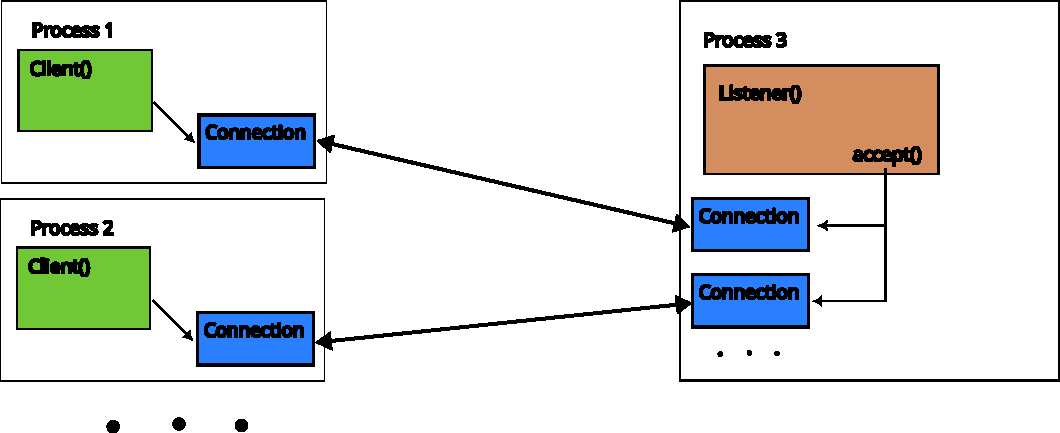
\includegraphics[width=\textwidth]{listener_client.pdf}
    \caption{Relationships between Listeners, Clients and Connections}
\end{figure}

The example below shows a simple echo server -- a server that simply sends back to the client what it receives. It will only accept connections from the local computer on the port 6000. First, the listener object is created using the \ls{with} statement, which is then used to start a separate thread which accepts the connections and responds to clients. The main thread will simply wait for the signal to quit. If we are supposed to quite, close the listener (we also need to unblock the \ls{accept()} which would wait forever) and quit. Note that the passwords are optional, if you do not specify the \ls{authkey} for the \ls{Listener}, you also do not have to specify it for \ls{Client}.

The client is in comparison much simpler. Simply connect to the listener with known address, port and password, and you can start sending and receiving data. Note that \ls{send()} and \ls{recv()} pickle and unpickle (recall pickling from \ls{.npy} files), so almost all Python-objects can be sent.

To test the example below, run \verb|python server.py| in one console and \verb|python client.py| in another.

\ls{server.py}:
\lstinputlisting{../example_code/ipc_server.py}

\ls{client.py}
\lstinputlisting{../example_code/ipc_client.py}

To allow connections from the network, simply specify the Listener address as \ls{''} (empty string) and the connect with the client to the IP address of the computer running the listener process. Note that pickling and unpickling in \ls{send()} and \ls{recv()} can lead to potential security issues, so it is best to use a password if accepting connections over the network.

\begin{exercise}
A server is running on computer with IP address \verb|<IP>|, on port \verb|<PORT>| with password \verb|<PASSWORD>|. This server is controlling a Pico by directly sending whatever string it receives to the pico and sending the response from the pico back.%
\end{exercise}

\verb|instrument_server.py|:
The code accepts the connections in a separate thread. For each connection it accepts, it starts a new client handler thread. All client handler threahds share the same pico, so we have to lock it appropriately before attempting communication, because another client can interrupt us at any moment. The server quits when it receives KeyboardInterrupt (Ctrl-C) 
\lstinputlisting{../example_code/instrument_server.py}

\subsubsection{Real use case in a lab}
In Fig.~\ref{fig:networking-usecase} is a photo of a single computer which controls three experiments connected to two different experimental setups. Each experiment belongs to a different student, who might need to run and modify their measurement Python scripts at the same time, so simple remote desktop sharing is not available.

We ended up using an instrument server similar to the simplified example above, which allowed the students to run the measurement scripts on any computer on the same network, even on their own laptops.

\begin{figure}
    \label{fig:networking-usecase}
    TODO
    \caption{Single computer controlling multiple experiments.}
\end{figure}

\newpage
\section{Solutions of differential equations}
\subsection{Initial value problems}
Initial value problems are differential equations of the form
\begin{equation}
    \label{eq:ivp}
    \diff{\bv y}{t} = \bv f(\bv y, t),
\end{equation}
where $\bv y$ is a vector, $t$ is the time and $\bf f$ is an arbitrary function together with the initial condition $\bv y(t=0) = \bv y_0$. Note that the equation is always written in the form of a first-order ordinary differential equation. However, differential equation of any order can be re-written as a first order equation by setting the vector $\bv y = (y(t), y'(t), y''(t), \dots)$. For example, a Newton's law of motion, $\ddot x = F/m$ would correspond to $\bv y = (x, \dot x)$ and $\bv f = (\dot x, F/m)$.

These types of equations are usually solved by \emph{time stepping}: given that we know $\bv y(t=0) = \bv y_0$, we calculate $\bv y(\dd t) \approx \bv y(0) + \bv f(\bv y(0), 0)\dd t$; $\bv y(2\dd t) \approx \bv y(\dd t) + \bv f(\bv y(\dd t), \dd t)\dd t$ $\dots$. This time stepping is called the \emph{Euler} method and generally requires a small time step to be accurate and numerically stable.\footnote{Numerical \emph{in}stability is the tendency of an error (i.e., the difference between the true solution and its numerical approximation) to oscillate wildly or grow to infinity.} There are many time stepping schemes that are more accurate and stable than the basic Euler method. The accuracy of the method is often quantified using the big-O notation, i.e., the Euler method is $O(\dd t)$, or a first-order method, which means that if we halve the time step $\dd t$, we also halve the error at every step. Very common are the explicit Runge-Kutta methods, of which the 4-th order version (with accuracy $O(\dd t^4)$) is probably the most common, i.e., if we halve the time step, the error decreases by factor 16.

The fourth-order Runge Kutta (RK4) calculate $y(t + \dd t)$ from $y(t)$ as
\begin{equation}
    \label{eq:RK4}
    y(t + \dd t) = y(t) + \frac{\dd t}{6}\left(k_1 + 2k_2 + 2k_3 + k_4\right),
\end{equation}
where
\begin{equation}
    \begin{aligned}
        k_1 &= f(y_t, t)\\
        k_2 &= f\left(y_t + \frac{1}{2}\dd t k_1, t + \frac{1}{2}\dd t\right)\\
        k_3 &= f\left(y_t + \frac{1}{2}\dd t k_2, t + \frac{1}{2}\dd t\right)\\
        k_4 &= f(y_t + k_3 \dd t, t + \dd t).
    \end{aligned}
\end{equation}
Notice that for each time step, the function $f$ has to be evaluated 4 times, and the calculation is about 4 times slower than the Euler method. There are also time stepping methods which instead of taking 4 times as long, the take-up 4 times as much space (e.g., Adams-Bashforth family of methods) which use the last four steps in the history of $y(t)$ to estimate the next step.

The RK4 method for a problem of type \eqref{eq:ivp} is implemented in \verb|SciPy| in \ls{scipy.integrate.solve_ivp()}. The \ls{solve_ivp()} expects the function $f(t, y)$, which takes the time and state vector and returns the time derivative of the state vector, the initial condition, and the time range where the evolution should be calculated.

The calculation can also watch for \emph{events} -- typically a signal, that a calculation should end. These are functions of time and the state vector which \emph{change sign} when the event occurs. An event can be made terminal (i.e., when even occurs calculation should stop) by simply setting the \ls{terminal} attribute of the function to \ls{True}. Remeber, functions are objects, and we can set their attributes as we please (similarly to \ls{self.attribute = value} when working with classes).

\textbf{Example}: Calculate the ballistic trajectory of a ball kicked under angle of 45$^\circ$ with initial velocities of 3 m/s along both $x$ and $y$ directions. The ballistic trajectory is the trajectory of a projectile thrown in a medium (e.g., air) which exerts nonlinear drag force on the motion of the form
\begin{equation}
    \bv F_d = -\frac{1}{2}A|\bv v|\bv v \rho \mathrm{CD},
\end{equation}
where $\bv v$ is the velocity of the projectile, $A$ is the area of the projectile projected facing the direction of motion, $\rho$ is the density of the medium and CD is the drag coefficient, $\mathrm{CD}\approx0.47$ for a ball.

\textbf{Solution:}
Full code is available in \ls{ivp_ballistic.py}. First, we import necessary modules and define the needed constants
\lstinputlisting[linerange={1-10}]{../example_code/ivp_ballistic.py}

Next we define the function $f$. We take the state vector $\bv x = (x, y, v_x, v_y)$ to represent both the position and velocity vectors. The function must return the time derivative of this 4-component state vector
\lstinputlisting[linerange={12-25}]{../example_code/ivp_ballistic.py}

Next we define the event that will indicate that the ball hit the ground and make it terminal, because we do not want the calculation to continue past this point
\lstinputlisting[linerange={30-34}]{../example_code/ivp_ballistic.py}

Now we have everything we need to calculate the ballistic trajectory. We set the calculation time range to $(0, 10)$, 10 being just arbitrary large time, the calculation will be stopped by the impact event. We also pass additional arguments, the drag coeffecient, through the usual \ls{args=} keyword argument. Finally, we also ask for a \ls{dense_output}, which will return an interpolation object (\ls{solution.sol} below) to represent the solution. This is useful, because \ls{solve_ivp} uses adaptive size of the time step $\dd t$ (i.e., when the derivatives are small and slowly-changing, the time step is bigger), so if we want an evenly sampled solution we have to interpolate it. With the returned solution, we use the time of the event to create an evenly sampled time array and return the interpolated trajectory.

Finally, we calculate the trajectory with and without air resistance and plot. We use slightly non-zero initial condition in the $y$ position to avoid triggering the event in the beginning.
\lstinputlisting[linerange={36-}]{../example_code/ivp_ballistic.py}

% \lstinputlisting{../example_code/ivp_ballistic.py}
\begin{center}
    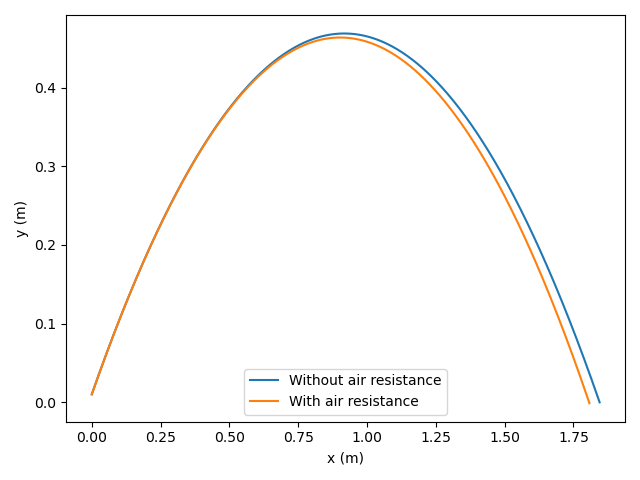
\includegraphics[width=0.6\linewidth]{ballistic.png}
\end{center}

\begin{exercise}
    Simulate the population dynamics of predators and prey (foxes $F$ and rabbits $R$) using the Lotka-Volterra model:
    \begin{equation*}
        \begin{aligned}
            \frac{\dd R}{\dd t} &= aR - bFR\\
            \frac{\dd F}{\dd t} &= dFR - cF
        \end{aligned}
    \end{equation*}
    with $a = 2/3$, $b = 4/3$ and $c = d = 1$. Plot $R(t)$ and $F(t)$ and the trajectory in phase space $R-F$.
\end{exercise}

\begin{exercise}
    Simulate the Lorenz system (the first properly studied example of deterministic chaos) given by equations
    \begin{equation*}
        \begin{aligned}
            \frac{\dd x}{\dd t} &= \sigma (y - x)\\
            \frac{\dd y}{\dd t} &= x(\rho - z) - y\\
            \frac{\dd z}{\dd y} &= xy - \beta z,
        \end{aligned}
    \end{equation*}
    with $\sigma = 10$, $\rho = 28$, and $\beta = 8/3$. Plot the $x$, $y$, $z$ trajectory in 3D space.
\end{exercise}

\begin{syntax}[3D plotting]
Matplotlib supports 3D plotting. On recent versions of matplotlib, a simple 3D plot of a line given by arrays \ls{x}, \ls{y}, and \ls{z} is very simple:
\begin{lstlisting}
fig3d = plt.figure()
ax3d = fig3d.add_subplot(projection='3d')
ax3d.plot(x, y, z, lw=0.5)
\end{lstlisting}
\end{syntax}

\subsection{Boundary value problems}
Boundary value problems are differential equations of the form
\begin{equation}
    \label{eq:bvp}
    F(\bv y, x) = 0
\end{equation}
where $F$ is some function that defines our problem that depends on the unknown function itself and its derivatives, $\bv y$ is the unknown function of $x \in [a,b]$ subject to boundary conditions $B(y_a, y_b) = 0$. Here the unknown function is a function of space, rather than time, and we need to know the solution "everywhere" at once. The numerical algorithms typically start from some initial guess and then iteratively optimize the solution $\bv y$ to fulfill the equation \eqref{eq:bvp} while maintaining the boundary conditions.

Solution of 1D (dimension of $x$) boundary value problems is implemented in \verb|SciPy| in \ls{scipy.integrate.solve_bvp}, which also allows for finding unknown parameters for which the solution can exist (see example below). For multi-dimensional problems, you typically have to use a dedicated package or write your own.

We will solve a simple example of a 1D Schr\"{o}dinger equation:\\
\textbf{Example} Calculate the wave functions and energy levels of a particle in inifinite potential well with additional potential $V(x)$ inside the well.

The states of a quantum particle are described with a stationary Schr\"{o}dinger equation
\begin{equation}
    \label{eq:sch}
    E\psi = -\frac{\hbar^2}{2m}\frac{\dd^2\psi}{\dd x^2} + V(x)\psi,
\end{equation}
where $m$ is the particle mass, $\psi$ is the particle wave function and $E$ is the energy. Calculate in "atomic units", $\hbar = 1$, $m=1$ and potential of the shape shown in Fig.~\ref{fig:potential}, i.e., $V(|x| > 1) = \infty$ and $V(|x| < 0.1) = 10)$ and $V=0$ elsewhere.
\begin{figure}[h!]
    \centering
    \label{fig:potential}
    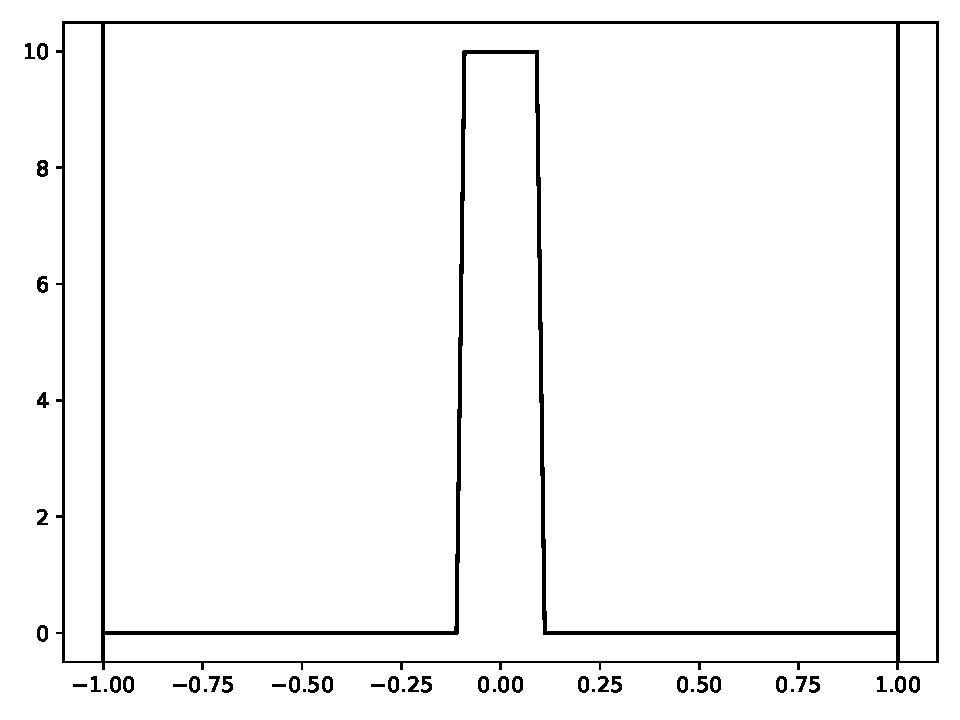
\includegraphics[width=0.5\linewidth]{sch_potential.pdf}
    \caption{Potential for the Schrödinger equation \eqref{eq:sch}.}
\end{figure}

\textbf{Solution:} The full code is available in \ls{bvp_schrodinger.py}. 

Begin by importing everything we need, define the constants \ls{w}, the width of the barrier and \ls{dh} the height of the barrier and the potential function itself. The infinite walls at $x=\pm 1$ will be taken care of by the boundary conditions.
\lstinputlisting[linerange={6-21}]{../example_code/bvp_schrodinger.py}

Next, define the function $F$ from \eqref{eq:bvp}. We rewrite the Schrödinger equation \eqref{eq:sch} to
\begin{equation}
    \frac{\dd^2\psi}{\dd x^2} = 2m(V(x) - E)\psi,
\end{equation}
and the unknown function $\bv y$ is then $(\psi, \dd \psi/\dd x)$. Finally, we also need to find the unknown parameter $E$. The function $F$ can depend on a vector of unknown parameters which \ls{solve_bvp()} finds together with the unknown function. In this case, this is just the energy.
\lstinputlisting[linerange={23-29}]{../example_code/bvp_schrodinger.py}

Next is the function representing the boundary conditions. This is an arbitrary function of the value of the unknown function at the boundaries and unknown parameters which the \ls{solve_bvp} maintain at zero. We have to return a vector of size 2 (i.e., the number of boundaries) + number of unknown parameters. In our case we simply want the wave function to be zero at the infinite wall. The third boundary condition is arbitrary, and its purpose is to simply ensure that the found solution is not identically 0.
\lstinputlisting[linerange={35-36}]{../example_code/bvp_schrodinger.py}
The number in the third condition is arbitrary, because the solution provided by \ls{solve_bvp} is not normalized.

Next we need to create the initial condition, both for the wave function and the energy, for the solver to optimize. Note that the original Schrödinger equation \eqref{eq:sch} has infinitely many solutions. To which solution \ls{solve_bvp()} actually converges is given by this initial condition. First we create the grid, i.e., points in space $x$ which are the argument of the wave function and create a simple estimate of wave function which is zero everywhere and non-zero in one off center point, in order to converge to a solution localized in one half of the potential well. Remember, the full initial condition is the wave function and its gradient, so \ls{y_0} is a 2D array of size 2 $\times$ length of \ls{x}.
\lstinputlisting[linerange={38-50}]{../example_code/bvp_schrodinger.py}

For the energy, we simply use the ground state energy of a particle in a simple infinite potential well.
\lstinputlisting[linerange={53}]{../example_code/bvp_schrodinger.py}

Finally, we have everything we need to call \ls{solve_bvp()}. Physically, the most interesting part is the probability of finding the particle at a position $x$, which is given by $|\psi(x)|^2$, so we plot that. To be exact, we should also normalize the wave function such that $\int |\psi(x)|^2 \dd x = 1$, however, since we are not calculating any quantum mechanical expectation values and are only interested in the shape of the distribution we plot it as it is, together with the potential and found energy.
\lstinputlisting[linerange={56, 65-74}]{../example_code/bvp_schrodinger.py}

\subsection{GPU acceleration}
Certain types of physical problems can be effeciently calculated on graphics cards (GPUs). These are problems which involve many independent calculations which can be run in parallel. A prototypical example is the gravitational $N$-body problem: calculate the motion of $N$ planets with equal masses $m$ that interact with each other via gravity only.

We will consider the 2D case for simplicity of plotting. The total force acting on planet $j = 1\dots N$ is
\begin{equation}
    \bv F_j = Gm^2\sum_{k\neq j}\frac{\bv r_k - \bv r_j}{|\bv r_k - \bv r_j|^2},
\end{equation}
where $G$ is the gravitational constant and $\bv r_k$ are the positions of the planets. The motion of the planet is then given simply by $m\ddot{\bv r_j} = \bv F_j$ and we could use \ls{solve_ivp()} as before. However, this problem becomes more scientifically interesting for large number of planets where \ls{solve_ivp()} would quicktly grind to a halt. Therefore we want to make use of fast GPUs.

The calculation will proceed again in steps: we will keep stored all positions and velocities of the planets. In every step, we will calculate the total force acting on all planets and then update positions and velocities via Euler stepping for simplicity. The calculation involves $N^2$ calculations of forces between planests which are independent of each other. Our goal is to use the GPU tu run these in parallel.

The full code is \verb|example_code/taichi/gravity.py|

\subsubsection{Setting up the environment}
We will be using the \ls{taichi} library to accelerate the computation from within Python, which has the advantage that it is rather simple, looks very much like standard Python code and allows using either GPU or CPU with the same code, so you can still try the code below even if you do not have a dedicated GPU in your computer. Taichi unfortunately requires Python version 3.10, which is most likely not the version you have installed. We do not want to clutter the system with multiple python versions, therefore we will use a \emph{virtual environment} to have an isolated installation of Python with its own version and packages.

The easiest way to manage virtual environments is with the \ls{uv} tool \url{https://docs.astral.sh/uv/getting-started/installation/}. On Windows, run the installation commands in the Windows Powershell.

Once \ls{uv} is installed, create an empty directory, let's call it "gravity", navigate to it in the command line and run
\begin{lstlisting}[language=bash]
uv venv -p 3.10
\end{lstlisting}
which will create the virtual environment with Python version 3.10. You shoud see output that looks similar to
\begin{verbatim}
Using CPython 3.10.16 interpreter at: /usr/bin/python3.10
Creating virtual environment at: .venv
Activate with: source .venv/bin/activate
\end{verbatim}
Activate the virual environment with the command from the last line. Your command line prompt shoud now show the virtual environment, e.g., on my linux machine
\begin{verbatim}
(gravity) emil@nt202 ~/gravity $
\end{verbatim}
This is a blank slate where we need to install all Python libraries we need. We will only need \ls{taichi} and \ls{matplotlib} (and their dependencies), which we can install simply using
\begin{lstlisting}
uv pip install taichi matplotlib
\end{lstlisting}
and now we have everything we need to start writing and running taichi code. However, we have to have the environment activated, otherwise we are using system-wide python which is not aware of the taichi library.

\subsubsection{Testing the installation}
TODO

\subsubsection{GPU Kernels}
Taichi allows us to offload specific functions to run on the GPU. These functions are handled differently from the rest of the Python code and are called \emph{kernels}. We will write two kernels, one for calculating the forces and one for the Euler stepping. We will store the data in numpy arrays -- this is not the fastest way (taichi can use memory more effeciently, see the taichi documentation for a more optimized version), but it is the simplest.

We import taichi and as it to use a GPU is possible using
\begin{lstlisting}
import taichi as ti
ti.init(ti.gpu)
\end{lstlisting}
This will use, in order of precedence, NVIDIA CUDA, Vulkan on AMD GPUs or the CPU.

The Euler stepping kernel looks like this
\lstinputlisting[linerange={49-59}]{../example_code/taichi/gravity.py}
We indicate that the function is a kernel using the \ls{ti.kernel} decorator. The function takes four arguments -- the positions of the planets \ls{rs}, the velocities \ls{vel} and accelerations \ls{acc}, which are numpy arrays of 64 bit floats of shape \ls{(N,2)} ($N$ planets and two coordinates) and the time step \ls{dt} which is a simple float.

Inside, the function look rather ordinary, however it does run inside the GPU and the outer-most for loop is in fact not a loop but iterations are executed in parallel as much as possible. There are some restrictions -- for example, you are not allowed to \ls{break} out of the outermost loop. The inner loop (\ls{for k in range(2)}) runs as an ordinary sequential for loop. We do not return anything, but rather modify the input arrays.

A more interesting kernel is the calculation of accelerations (or forces), which looks like this
\lstinputlisting[linerange={14-46}]{../example_code/taichi/gravity.py}

Our problem is relatively simple, so-called \emph{embarrassingly parallel}\footnote{This is an actual term used in the computer science.} because the calculations are entirely independet of each other. GPUs are capable of running many task in parallel quickly because they do not allow for synchronisation (or only in a very limited form). This means, that despite running many things in parallel, we do not have any mechanism similar to \ls{Lock()} from multithreading. Therefore, if the iterations of the loop depend on each other, avoiding race conditions becomes somewhat more complicated. For example, imagine some planets are made of matter and some of anti-matter and if they get too close to each other they annihilate. We could implement this this for example as
\begin{lstlisting}
for j in range(N):
    for k in range(N):
        if planet_is_alive(j) and planet_is_alive(k):
            if distance(j,k) < annihilation_distance:
                annihilate(j,k)
\end{lstlisting}
This would be OK if the loops are sequential. However, when the outermost loop runs in parallel, we could get to a situation where we have palents $j=1$ (matter) and $k=2, 3$ (anti-matter) which are all close to each other. Since the check on line 3 might be using old data, we could end up running both \ls{annihilate(1,2)} and \ls{annihilate(1,3)} and thus increasing the ratio of matter to anti-matter in the universe.

\subsubsection{Using the kernels}
To represent the state of the simulation -- the positions and velocities of the planets and the time we will use a simple class. As an initial condition we will random positions in 2D with normal distribution around origin and solid body rotation for velocities with some initial angular velocity. The class will have only two methods, which call the two kernels we wrote above,
\lstinputlisting[linerange={61-88}]{../example_code/taichi/gravity.py}

Finally, we create a simulations with 5000 planets, plot a real-time animation using matplotlib and periodically save a picture
\lstinputlisting[linerange={91-130}]{../example_code/taichi/gravity.py}

After about a minute of runtime on Intel Core i7-7700 CPU (a fairly old CPU) the initial gaussian distribution of the planets develops some interesting structure
\begin{center}
    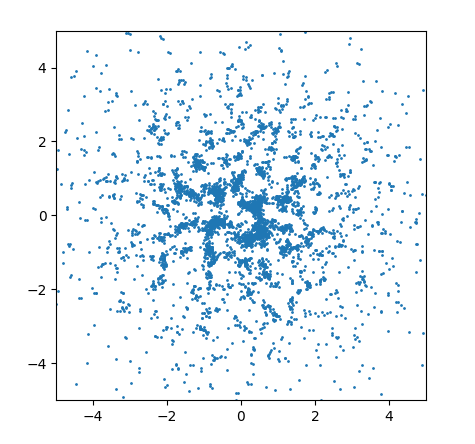
\includegraphics[width=0.5\linewidth]{gravity.png}
\end{center}

\newpage
\section{What didn't fit}

\subsection{PID algorithm}
TODO

\subsection{Symbolic mathematics}
TODO: sympy


% \section{Image processing}
% TODO, \ls{opencv}

% \section{Some AI crap?}
% TODO \ls{scikit-learn}

\newpage
\appendix
\section{Linear Harmonic Oscillator}
\label{sec:lho}
A linear harmonic oscillator with friction is described by a dynamical equation
\begin{equation}
    \label{eq:lho}
    \ddot x + \omega_0^2 x + \gamma\dot x = F(t)/m,
\end{equation}
where $m$ is the oscillator mass, $\omega_0$ is the resonance frequency, $\gamma$ the friction coefficient and $F(t)$ the external force. Assuming that the force has the form $F(t) = \Re(\tilde F e^{i\omega t})$ and that the solution has the form $x(t) = \Re(\tilde x e^{i\omega t})$ (or applying the Fourier transform to both sides of the equation) we get by simple rearranging
\begin{equation}
    \tilde x = \frac{1}{m}\frac{\tilde F}{\omega_0^2 - \omega^2 + i\gamma\omega} = \chi(\omega)\tilde F,
\end{equation}
where $\chi(\omega)$ is called susceptibility.

Since Eq.~\ref{eq:lho} is a linear equation, the response to a sum of forces will be the sum of responses to each force.

\section{Setting up communication with instruments}
\label{sec:pico}
We will use VISA library to talk to instruments. To talk to the Raspberry Pi Pico we will use a Python implementation of the library, for which we need to install at least \ls{pyvisa, pyvisa-py} and \ls{pyusb} using
\begin{lstlisting}[language=bash]
    pip install pyvisa pyvisa-py pyusb
\end{lstlisting}
which you should run in a command line which is aware of the python installation (e.g., Anaconda Propmt if on Windows with Anaconda Python distribution). On Linux you should also add yourself to the \ls{dialout} group (do not forget the \ls{-a} switch),
\begin{lstlisting}[language=bash]
    sudo usermod -a <your username> -G dialout 
\end{lstlisting}
and log out and log in.

To test the installation run the \ls{pyvisa-info} from the command line. A bunch of information should be printed out, look for line that looks like
\begin{lstlisting}
    USB INSTR: Available via PyUSB (1.2.1). Backend: libusb1
\end{lstlisting}

Next, create a Python script \ls{list_resources.py} with the following code
\lstinputlisting{../example_code/list_resources.py}
and run it. It should list either nothing or a few COM (or tty on Linux) ports. Next connect the Pico and run the program again, a new address should appear, that is the address we will use to communicate with the Pico.

Next, run the following code, replacing \ls{"ASRL/dev/ttyACM0::INSTR"} with the address you found in the previous step.
\lstinputlisting{../example_code/idn.py}
The program should print "PICO" and quit without error.

For more full-featured implementation of visa you may consider the implementation from \href{https://www.ni.com/en/support/downloads/drivers/download.ni-visa.html#548367}{National Instruments} (NI). The NI-VISA library is free, but not open source and registration is required. Linux support is also limited to out-of-date kernels.

\subsection{Supported commands}
\begin{tabular}{p{15cm}}
    \textbf{*IDN?}\\
    Query identification string. Should reply PICO.
    \\\hline
    \textbf{:LED n m}\\
    Turns the LED $n$ on (m=1) or off (m=0). The LED number $n = 0 \dots 4$, red LED is 0.
    \\\hline
    \textbf{:READ:P?}\\
    Reads the pressure in Pa.
    \\\hline
    \textbf{:READ:T?}\\
    Returns the temperatures as $100T$ where $T$ is the temperature in $^\circ$C.
    \\\hline
    \textbf{:READ:PT?}\\
    Reads both temperature and pressure
    \\\hline
    \textbf{:READ:ACC?}\\
    Reads the accelerometer. Returns three space-separated values in the range -32768 to 32768 which maps to $-2g$ to $2g$.
    \\\hline
    \textbf{:READ:GYR?}\\
    Reads the gyroscope. Returns three space-space separated values in the range -32768 to 32768 which maps to $-500^\circ$/s to $500^\circ$/s.
\end{tabular}

\subsection{Hacking the firmware}
The source code of the program running on the Pico is available \href{https://bitbucket.org/emil_varga/picolab/src/master/}{here}. To compile it, you need to set up Pico SDK, follow the instructions \href{https://www.raspberrypi.com/documentation/microcontrollers/c_sdk.html}{here}.

Alternatively you can use MicroPython to run Python code on the Pico directly, follow the instructions \href{https://www.raspberrypi.com/documentation/microcontrollers/micropython.html#what-is-micropython}{here} for set up. 

LEDs are wired to GP0 -- GP4 pins and the sensors are connected to the I2C0 controller on pins 16 and 17.
\end{document}
